\chapter{NOAH}
\label{chpt:noah}

\epigraph{\singlespacing%
The power of doing any thing with quickness is always much prized by the possessor, and often without any attention to the imperfection of the performance.%
}{--- \textsc{Jane Austen}, \textit{Pride and Prejudice}}

This final chapter describes my work on \textit{NOAH} (NMR by Ordered Acquisition using \proton{} detection) \textit{supersequences}, pulse sequences which record multiple 2D datasets (\textit{`modules'}) in the time required for one.
This is an attractive NMR technique for several reasons: the time savings are clearly a key factor, but the flexibility of being able to combine almost any set of modules also makes NOAH supersequences applicable to a variety of contexts.

I begin by introducing the concepts underlying NOAH supersequences, as well as a general discussion of the time savings (and sensitivity per unit time benefits) thus realised.
I then describe the GENESIS (GENEration of Supersequences In Silico) website, written by me, which allows users to generate Bruker pulse programmes for almost every imaginable NOAH supersequence.
After this, my work on various aspects of the actual sequences themselves is described, with a special focus on newly developed and/or improved modules.
Finally, the design of `parallel' supersequences, which comprise multiple interleaved supersequences, is discussed.

This work was done in close collaboration with \EK{} (Bruker UK).
However, all results and analysis shown in this chapter are mine.
The work in this chapter forms the subject of several publications:

\begin{itemize}
    \item \fullcite{Yong2021JMR}
    \item \fullcite{Kupce2021JACSA}
    \item \fullcite{Yong2022AC}
    \item \fullcite{Yong2023CC}
\end{itemize}

The material in the introductory sections also closely follow two reviews which I have contributed to:
\begin{itemize}
    \item \fullcite{Kupce2021NRMP}
    \item \fullcite{Yong2023RSCBook}
\end{itemize}

\clearpage

\section{Introduction}
\label{sec:noah__introduction}

The characterisation of small molecules and biomolecules by NMR spectroscopy relies on a suite of standard 2D NMR experiments, which seek to detect heteronuclear scalar couplings (e.g.\ HSQC and HMBC), homonuclear scalar couplings (e.g.\ COSY and TOCSY), or through-space interactions (e.g.\ NOESY and ROESY).
Although 2D experiments provide far superior resolution and information content compared to 1D spectra, they also require substantially longer experiment durations, as the indirect dimension must be constructed through the acquisition of many $t_1$ increments.
This problem is further exacerbated by the fact that structural elucidation or verification often necessitates the acquisition of several different 2D experiments.

The acceleration of 2D NMR has thus proven to be a popular area of research.
We may broadly categorise existing techniques into two classes: firstly, those which seek to directly speed up the acquisition of \textit{individual} 2D spectra, and secondly, \textit{multiple-FID} experiments which aim to collect two or more 2D spectra in the time required for one.%
\footnote{These are by no means mutually exclusive: many of the techniques here can be combined to provide even greater efficiency.}
The former category includes methods such as 
\acf{nus}\autocite{Barna1987JMR,Kazimierczuk2010PNMRS,Mobli2014PNMRS,Kazimierczuk2015MRC},
fast pulsing (i.e.\ shortening of recovery delays)\autocite{SchulzeSunninghausen2014JACS,Schanda2006JACS,Kupce2007MRC,Schanda2009PNMRS},
ultrafast NMR\autocite{Frydman2002PNASUSA,Pelupessy2003JACS,Frydman2003JACS,Tal2010PNMRS,Gouilleux2018ARNMRS,Kupce2021NRMP},
Hadamard encoding\autocite{Kupce2003JMR,Kupce2003PNMRS},
and spectral aliasing\autocite{Jeannerat2000MRC,Bermel2009JACS,Njock2010C,Jeannerat2011eMR};
whereas the latter encompasses 
time-shared NMR\autocite{Nolis2007ACIE,Parella2010CMR},
multiple-receiver NMR\autocite{Kupce2006JACS,Kupce2008JACS,Kovacs2016MRC},
and---of course---NOAH supersequences\autocite{Kupce2017ACIE,Kupce2021PNMRS,Kupce2021NRMP}.

The scope of this introductory section will be limited to only NOAH supersequences.
However, many of these techniques are closely related, and I will introduce concepts from elsewhere as needed.
It should be noted that there are several other multiple-FID experiments which, while not explicitly advertised as such, are conceptually identical to NOAH experiments.\autocite{Nagy2019CC,Nagy2020JMR,Nagy2021ACIE,Timari2022CC}
I do not discuss these here.

\subsection{Time savings and sensitivity analyses}
\label{subsec:noah__snr}


\subsubsection{Time savings in the sampling-limited regime}

\begin{figure}[htb]
    \centering
    
\includegraphics[]{noah/timings.png}%
    {\phantomsubcaption\label{fig:noah_timings_noah_sc}}%
    {\phantomsubcaption\label{fig:noah_timings_conv_s}}%
    {\phantomsubcaption\label{fig:noah_timings_conv_c}}%
    \caption[Comparison of NOAH and conventional 2D experiments]{
        \textbf{(\subref*{fig:noah_timings_noah_sc})} \noah{S,C} supersequence, comprising HSQC and COSY modules (see \cref{tbl:noah_modules} for an explanation of the single-letter module codes used).
        \textbf{(\subref*{fig:noah_timings_conv_s})} `Conventional' echo--antiecho HSQC (the same as in \cref{fig:hsqc_etgp}).
        \textbf{(\subref*{fig:noah_timings_conv_c})} `Conventional' COSY.
        The timings referred to in the text are highlighted for all three experiments; $d_1$ for each experiment is assumed to be the same.
        Note that the lengths are not to scale: $d_1$ is typically far longer than $\taups$ and $\tauacq$.
    }
    \label{fig:noah_timings}
\end{figure}


The duration of an NMR experiment, $\tauexp$, can be expressed as a sum of its parts:
\begin{equation}
    \label{eq:exp_duration_2d}
    \tauexp = \taups + \tauacq + d_1,
\end{equation}
where $\taups$ is the time required for the pulse sequence itself (typically several milliseconds), $\tauacq$ is the acquisition time (several hundred milliseconds), and $d_1$ is the recovery delay (one or more seconds).
These timings are illustrated in \cref{fig:noah_timings} for a NOAH supersequence formed from two modules (HSQC and COSY).
The \textit{time-saving factor} for a NOAH supersequence, as compared to a series of conventional standalone experiments, is denoted $\rho_t$ and may be expressed as:
\begin{equation}
    \label{eq:rho_t}
    \rho_t
    = \frac{\sum_i \tauconv^{(i)}}{\tauNOAH}
    = \frac{{\sum_i (\taups^{(i)} + \tauacq^{(i)} + d_1^{(i)})}}{d_1 + \sum_i (\taups^{(i)} + \tauacq^{(i)})},
\end{equation}
where $\tauNOAH$ is the duration of the NOAH supersequence, $\tauconv$ is the duration of a conventional experiment, and the superscript $(i)$ represents the $i$-th module or conventional experiment being acquired.%
\footnote{This notation implies that $\taups^(i)$ is the same in both the conventional experiment and the corresponding NOAH module. This is not strictly true: NOAH modules are often modified from the original, as will be explained shortly. However, the differences in timings are so minute that they can be completely ignored, especially when compared against $d_1$.}
The sum runs from $i = 1$ to $N$, where $N$ is the number of modules.
If we assume that $d_1^{(i)} = d_1$ is the same for all $N$ conventional experiments and the supersequence, then in the limit where
\begin{equation}
    \label{eq:d1_limit}
    d_1 \gg \sum_i \taups^{(i)} + \tauacq^{(i)},
\end{equation}
we have that $\rho_t \to Nd_1/d_1 = N$, i.e.\ an $N$-fold time saving.

This statement makes plenty of assumptions, and is not entirely valid in practice.
For example, \textit{each} $\tauacq$ is often around 5--10\% of $d_1$, so is not entirely negligible, especially when $N$ is larger.
Furthermore, for some modules, $\taups$ itself can be substantial: most notable is the NOESY module, which contains a mixing time of several hundred milliseconds.
(HMBC, TOCSY, and ROESY modules are also lesser offenders.)

These factors serve to reduce $\rho_t$ from its idealised value of $N$; generally, this deviation is larger as $N$ increases, because \cref{eq:d1_limit} becomes less and less valid.
Despite this, it remains true that the time savings are approximately proportional to $N$, as will be shown in \cref{tbl:noah_sensitivities}.

For relatively concentrated samples, where sensitivity is not an issue, these time savings are the sole relevant point.
In this \textit{sampling-limited regime}, the minimum 2D experiment duration is dictated purely by the number of $t_1$ increments needed to obtain sufficient resolution in the indirect dimension, as well as the minimum phase cycle required for artefact suppression.%
\footnote{With modern gradient-enhanced experiments, the minimum phase cycle may not even be a `cycle', as one scan per increment may suffice; see also \cref{fig:hsqc_comparison}.}
NOAH supersequences are identical to conventional experiments in both these aspects, but come with the added benefit of time savings.
The development of modern NMR instrumentation (such as high-field magnets and cryogenic probes) plays an important role in extending the sampling-limited regime to ever lower concentrations.


\subsubsection{Sensitivity comparisons}

However, the opposite \textit{sensitivity-limited regime} is still very commonly encountered.
This can happen, for example, with naturally insensitive experiments (e.g.\ ADEQUATE), low-field benchtop NMR, or most simply, dilute samples.%
\footnote{If the SNR factor $A^{(i)}$ as discussed below is \textit{very small}, then it is possible that even concentrated samples may be shifted into the sensitivity-limited regime. This is never really the case in practice, though, as the case studies in \cref{subsec:noah__case_studies} will illustrate.}
In such cases, the benefits of NOAH supersequences must be much more carefully considered: in particular, it becomes mandatory to compare the SNRs of the NOAH modules and conventional experiments.
To do so, we define for each module an \textit{SNR factor} $A$, which is the SNR of the NOAH module divided by the SNR of a conventional experiment, acquired with the same parameters.%
\footnote{The relative SNR will likely vary from peak to peak in the spectrum, and $A$ should in theory be quoted either as an average over all peaks, or as a range.
This is what I have done in this thesis.
Furthermore, the exact values calculated for $A$ will depend on the sample used for the comparison.
Any values given here should therefore be assumed to be valid only for similar samples.
Of course, my hope is that the samples chosen are reasonably representative of `typical' organic molecules.}
The SNR factor of the $i$-th module in a supersequence may be denoted as $A^{(i)}$.

In general, we have that $A \leq 1$, because (as will be explained in \cref{subsec:noah__magpools}) NOAH modules frequently contain small modifications with respect to conventional experiments.
For sensitivity-limited samples, we must balance these losses against the time savings obtained, by defining a \textit{gain in sensitivity per unit time}, $\varepsilon$ as
\begin{equation}
    \label{eq:varepsilon_i}
    \varepsilon = A \sqrt{\rho_t}.
\end{equation}
Here, the square root accounts for the fact that SNR scales only as the square root of the number of scans, or equivalently, the number of times the experiment can be repeated in a given time.
If $\varepsilon^{(i)} > 1$, as is frequently the case, this means that the NOAH supersequence provides greater sensitivity per unit time in the $i$-th module compared to a standalone experiment.
Equivalently, performing a NOAH experiment allows data of sufficient sensitivity to be obtained in less time.%
\footnote{The use of $\varepsilon = A\sqrt{\rho_t}$ ignores the fact that experiments can only be repeated an integer number of times. For example, if $\rho_t = 2.5$, this does not necessarily imply that the NOAH experiment can be repeated $2.5$ times more to get a $\sqrt{2.5} \approx 1.58{\times}$ boost in sensitivity. However, it is impossible to account for this in a general manner, so I will ignore it.}


\subsubsection{Time savings in the sensitivity-limited regime}

An important---yet often ignored---caveat with sensitivity-limited samples is that the time savings obtained are not \textit{truly} on the order of $N$ as advertised above.
This is because each module in a NOAH supersequence is run with the same number of scans.
In contrast, with conventional experiments, it is common to run more insensitive experiments with a larger number of scans but to use fewer scans for sensitive experiments.
In this case, the \textit{effective} time savings provided by NOAH experiments are smaller:
\begin{equation}
    \label{eq:rho_t_eff}
    \rhoteff
    = \frac{\sum_i \tauconv^{(i)}}{\tauNOAH}
    = \frac{{\sum_i S^{(i)}(\taups^{(i)} + \tauacq^{(i)} + d_1^{(i)})}}{Sd_1 + S\sum_i (\taups^{(i)} + \tauacq^{(i)})},
\end{equation}
where each standalone experiment is acquired with $S^{(i)}$ scans, and the NOAH experiment with $S$ scans.
We could also analogously define $\vareeff = A\sqrt{\rhoteff}$.

Typically, $S$ is simply the largest of the $S^{(i)}$, as this ensures sufficient data quality for the most insensitive module in the supersequence.
This means that generally, $\rhoteff < \rho_t$.
In such a situation, it is probably more appropriate to describe a NOAH supersequence as `measuring the most insensitive module and getting the others for free'.
Indeed, in the extreme case where $S = S^{(i)} \gg S^{(j\neq i)}$, then `the other' modules require almost no time to measure (relative to the least sensitive, $i$-th, module), and $\rhoteff$ tends towards 1, meaning that even the time-saving utility of NOAH vanishes.
A corollary of this is that NOAH supersequences are generally most useful when constructed from modules which have similar intrinsic sensitivities and hence similar $S^{(i)}$'s: this is not necessary in the sampling-limited regime where $S^{(i)} = S$ for all $i$ (and \cref{eq:rho_t_eff} simply reduces to \cref{eq:rho_t}), but is crucial in the sensitivity-limited regime.

As the reader will no doubt appreciate by now, the comparison of NOAH and conventional spectra is fraught with subtleties.
In fact, it is very much possible to construct yet more edge cases which challenge the framework used in this analysis.
For example, one may not want to acquire all the individual spectra `conventionally': for example, NUS may be used for an HSQC experiment but not for others; or $d_1$ may be varied for different experiments.
These will have an impact on both the durations of the experiments, as well as their sensitivities.
To make any meaningful comparisons or generalisations, it is therefore necessary to restrict the discussion to values of $\rho_t$, $A$, and $\varepsilon$, which can be objectively calculated.
These should, however, be read with the understanding that other factors may, depending on the context, lead to \textit{some}---but never a \textit{complete}---decrease in the utility of NOAH experiments.

\subsection{Magnetisation pools}
\label{subsec:noah__magpools}

Having gotten this relatively dry material out of the way, I now turn to exactly how NOAH supersequences are constructed.
Ordinarily, if the recovery delay is removed from an NMR experiment, its sensitivity will be greatly reduced because insufficient magnetisation will have recovered between repetitions; or in other words, $A^{(i)}$ will be very small.
Such experiments would only really be useful well in the sampling-limited regime.

The key to avoiding this in NOAH supersequences is to make sure that \textit{each module samples a different source of magnetisation}.
For example, an HSQC module can be designed to only sample magnetisation of protons directly bonded to the 1.1\%-natural abundance \carbon{}, and leave all other proton magnetisation untouched.
Immediately following this, the remainder of the proton magnetisation can then be used to record (say) a COSY module, without needing a separate recovery delay.
Using the notation of Orts and Gossert\autocite{Orts2018M}, the magnetisation of \carbon{}--bound protons is denoted as \magn{C}, and the magnetisation of protons \textit{not} bonded to \carbon{} is denoted as \magnnot{C}.
Protons not directly bonded to NMR-active heteronuclei are labelled \magnnot{X}, and will often be referred to as `bulk' magnetisation, since (in natural-abundance samples) the majority of protons fall into this category.

Most standard 2D experiments do not preserve unused magnetisation but instead dephase it through CTP gradient selection; thus, NOAH modules often require some modifications compared to standard experiments.
For example, compared to the echo--antiecho HSQC (discussed in \cref{subsec:theory__hsqc_ea}), the NOAH HSQC module\autocite{Kupce2017ACIE} adds an extra CTP gradient so that the bulk magnetisation is refocused and ultimately returned to the $+z$ equilibrium state (\cref{fig:noah_sb_po_s}).
(This is largely identical to the `symmetrised' ASAP-HSQC experiment\autocite{SchulzeSunninghausen2017JMR}.)

\begin{figure}[htb]
    \centering
    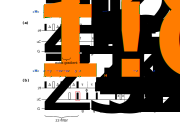
\includegraphics[]{noah/hsqc_hmbc_prodops.png}%
    {\phantomsubcaption\label{fig:noah_sb_po_s}}%
    {\phantomsubcaption\label{fig:noah_sb_po_b}}%
    \caption[NOAH HSQC and HMBC modules with product operator analysis]{
        \textbf{(\subref*{fig:noah_sb_po_s})} 
        NOAH HSQC module.
        \textbf{(\subref*{fig:noah_sb_po_b})} 
        NOAH HMBC module.
        The \ang{90} pulse highlighted in red is described in \cref{subsec:noah__hmbc}.
        Delays are set as: $\Delta = 1 / (4 \cdot \oneJ{CH})$; $\Delta_\text{LR} = 1 / (2 \cdot \nJ{CH})$; $\tau_1 = 1 / (2 \cdot \oneJ{CH,\text{max}})$; $\tau_2 = 1 / (2 \cdot \oneJ{CH,\text{min}})$ (see also \cref{subsec:poise__hmbc} for the LPJF).
        Phase cycling is performed with $\phi_1 = (x, -x)$, $\phi_2 = (x, x, -x, -x)$, and $\phi_\text{rec} = (x, -x, -x, x)$.
        Gradient amplitudes are $(g_1, g_2, g_3, g_4, g_5) = (80\%, \pm 40.2\%, 15\%, -10\%, -5\%)$.
        Product operator analysis is provided above both modules for both the \magn{C} and \magnnot{C} magnetisation pools; the notation for this is explained in the \textit{Preface}.
    }
    \label{fig:noah_sb_po}
\end{figure}

Sometimes, the modifications required are more extensive, as in the HMBC module.
If this module is followed by an HSQC module (or any other module which draws on \magn{C} magnetisation), the initial \ang{90} excitation pulse must be replaced with a $zz$-filter (\cref{fig:noah_sb_po_b}).
This performs an \textit{isotope-selective rotation} in that \magn{C} magnetisation is stored along the $z$-axis, but \magnnot{C} magnetisation is excited (and subsequently detected).
In general, sequences which are thus modified have lower sensitivities (i.e.\ $A < 1$) than the `original' sequences from which they were derived.
This is partly because of imperfect manipulation of magnetisation by the extra pulse sequence elements, and also increased losses due to relaxation during these extended sequences.

In contrast, modules placed towards the \textit{end} of a supersequence do not need to be modified, as they do not need to preserve any magnetisation.
This includes virtually all homonuclear modules, which are allowed to simply consume any remaining magnetisation.
Although this makes their implementation very straightforward, in general these modules will \textit{also} suffer some losses in sensitivity, because the preceding modules do not perfectly retain all magnetisation.

Thus, in general, it is not possible for any module in a NOAH supersequence to have $A = 1$, unless it is placed first in the supersequence \textit{and} has not undergone any modifications.%
\footnote{Of course, this also depends on exactly \textit{what} standalone experiment the NOAH supersequence is being compared against. Sometimes, in the literature, the NOAH experiment has been compared against its constituent modules acquired in a standalone fashion; in this case, the first module will always have $A = 1$. This tells us how much we gain through the act of concatenating modules, but is less meaningful in the `real world' where one is interested in how useful NOAH is relative to `typical' optimised 2D experiments. I therefore prefer to make comparisons against standard-library sequences.}
Such cases are very rare, and it is thus necessary to accept some decreases in $A$, which are often fairly small (on the order of 10--20\%).
In the sampling-limited regime, sensitivity is not at a premium and this is often perfectly tolerable.
In the sensitivity-limited regime, the full time savings $\rho_t$ cannot be realised, but since $\varepsilon$ is still typically larger than 1, there is still an overall boost in sensitivity per unit time.

\subsection{Case studies}
\label{subsec:noah__case_studies}

Using all of the concepts described in the previous sections, we now look at a few `typical' supersequences to understand their construction.
Before beginning, a quick note about the nomenclature of NOAH supersequences is warranted.
Supersequences are labelled by the number of modules $N$, plus a series of single-letter codes corresponding to the identity and ordering of the modules involved (\cref{tbl:noah_modules}).
Occasionally, superscripts or subscripts are used to qualify the modules involved.%
\footnote{With the increasing number of modules, and the variety of modern NMR experiments which could be incorporated into NOAH supersequences, keeping these abbreviations short yet meaningful has been a challenge.}
Thus, a NOAH supersequence containing three modules---say \nitrogen{} HMQC, \carbon{} HSQC, and CLIP-COSY---would be referred to as a \noah{Mn,S,Cc}.
\Cref{tbl:noah_sensitivities} provides values of $\rho_t$ and $A$ for the example supersequences used in this section; these values which will be rationalised in the text which follows.

\begin{table}[!ht]
    \begin{tabular}{cccccc}
        \toprule
        \multicolumn{2}{c}{\textbf{\proton{}--\nitrogen{} modules}}  &
        \multicolumn{2}{c}{\textbf{\proton{}--\carbon{} modules}}    &
        \multicolumn{2}{c}{\textbf{\proton{}--\proton{} modules}}   \\
        \cmidrule(lr){1-2}
        \cmidrule(lr){3-4}
        \cmidrule(lr){5-6}
        Module & Code        & Module     & Code           & Module     & Code       \\
        \midrule
        HMQC   & \noah*{Mn}  & HSQC       & \noah*{S}      & COSY       & \noah*{C}  \\
        HSQC   & \noah*{Sn}  & seHSQC     & \noah*{Sp}     & CLIP-COSY  & \noah*{Cc} \\
        seHSQC & \noah*{Spn} & HSQC-TOCSY & \noah*{St}     & DQF-COSY   & \noah*{D}  \\
        HMBC   & \noah*{Bn}  & HSQC-COSY  & \noah*{Sc}     & TOCSY      & \noah*{T}  \\
               &             & 2BOB       & \noah*{O}      & NOESY      & \noah*{N}  \\
               &             & HMBC       & \noah*{B}      & ROESY      & \noah*{R}  \\
               &             & ADEQUATE   & \noah*{A}      & PSYCHE     & \noah*{P}  \\
               &             &            & \hspace{1.5cm} & TSE-PSYCHE & \noah*{Pt} \\
               &             &            &                & PSYCHE 2DJ & \noah*{J}  \\
        \bottomrule
    \end{tabular}
    % The hspace is to make the two subcolumns look more balanced.
    \caption[List of single-letter NOAH module codes]{
        A (non-exhaustive) list of single-letter module codes for NOAH modules.
        In the literature, the \nitrogen{} HMQC module has been referred to simply by `M', since the HSQC module is preferred for \proton{}--\carbon{} correlations.
        In this thesis, I include the subscript N throughout to avoid any ambiguity.
    }
    \label{tbl:noah_modules}
\end{table}

\begin{table}[!ht]
    % data are in lab book: noah-misc/220224/
    \begin{tabular}{ccccccccc}
        \toprule
        \textbf{Entry} & \textbf{Sequence} & $\symbf{\tau}_{\symbf{NOAH}}$ & $\symbf{\rho}_{\symbfit{t}}$ & \multicolumn{5}{c}{$\symbfit{A}$} \\
        \cmidrule(lr){5-9}
        & & & & HMBC & seHSQC & HSQC & COSY & TOCSY \\
        \midrule
        1 & \noah*{S,C}         & 15 min 0 s  & 1.87 &      &      & 0.97 & 0.90 &      \\
        2 & \noah*{S,C,T}       & 16 min 25 s & 2.60 &      &      & 1.01 & 0.99 & 0.79 \\
        3 & \noah*{B,S}         & 15 min 40 s & 1.82 & 0.93 &      & 0.87 &      &      \\
        4 & \noah*{S,B}         & 15 min 35 s & 1.83 & 0.99 &      & 0.96 &      &      \\
        5 & \noah*{B,S,C,T}     & 17 min 48 s & 3.22 & 0.95 &      & 0.90 & 0.36 & 0.28 \\
        6 & \noah*{B,Spn,S,C,T} & 18 min 57 s & 3.74 & 0.95 & 0.71 & 0.66 & 0.38 & 0.30 \\
        7 & \noah*{Spn,B,S,C,T} & 18 min 56 s & 3.75 & 0.76 & 0.79 & 0.74 & 0.33 & 0.26 \\
        \bottomrule
    \end{tabular}
    \caption[Sensitivity and time-saving analyses of several NOAH supersequences]{
        Sensitivity and time-saving analyses of several typical NOAH supersequences.
        All experiments were acquired with 2 scans per increment, 256 $t_1$ increments, an acquisition time of \qty{67}{\ms}, and a recovery delay of \qty{1.5}{\s}.
        The HMBC module used here includes the extra \carbon{} \ang{90} pulse described later in \cref{subsec:noah__hmbc}: this has no significant impact on the SNR, and is only mentioned as a technicality.
        The \nitrogen{} seHSQC module is that described in \cref{subsec:noah__sehsqc_n}.
        The CT module here was run with States indirect-dimension quadrature detection, and the individual C module (in entry 1) with echo--antiecho.
        The following Bruker library sequences were used as the `conventional' experiments: \texttt{hmbcetgpl2nd}, \texttt{hsqcetf3gpsi2}, \texttt{hsqcetgpsp.2}, \texttt{cosygpqf}, and \texttt{dipsi2gpphzs}.
        \datacode{7Z-220224}
    }
    \label{tbl:noah_sensitivities}
\end{table}

\subsubsection{\noah{S,C}: HSQC + COSY}

We begin with perhaps the simplest example of a NOAH supersequence, one containing the HSQC and COSY modules: this is labelled as a \noah{S,C} experiment (entry 1, \cref{tbl:noah_sensitivities}).
Using the implementation shown in \cref{fig:noah_sb_po_s}, the HSQC module only samples \magn{C} magnetisation, and leaves \magnnot{C} magnetisation along the $+z$-axis.
This modification to the HSQC module is very small, so its sensitivity is practically unaffected as compared to a `standard' HSQC ($A = 0.97$).
Furthermore, the COSY module retains \textit{most} of its sensitivity ($A = 0.90$).
The small loss here is because the HSQC module does not \textit{perfectly} preserve the \magnnot{C} magnetisation: for example, evolution of homonuclear couplings as well as relaxation occur during the HSQC pulse sequence, both of which were ignored in the product operator analysis of \cref{fig:noah_sb_po_s}.

Furthermore, the value of the time-saving factor, $\rho_t = 1.87$, is very close to the theoretical limit of $N = 2$.
This reflects the fact that the pulse sequence itself, $\tau_{\symup{ps}}$, is fairly short for both the HSQC and COSY modules; the deviation therefore chiefly arises from the acquisition time, $\tau_{\symup{acq}}$.
In all respects, this is therefore an example of an `ideal' NOAH supersequence, where the combination of two modules provides almost $2\times$ time savings without compromising on sensitivity.

It is worth pointing out that the order of the modules cannot be reversed: the COSY module cannot be (easily) modified to preserve \magn{C} magnetisation.
In a hypothetical \noah{C,S} supersequence, the later HSQC module would only be able to use magnetisation recovered during the COSY FID, leading to a substantial decrease in sensitivity.

\begin{figure}[!ht]
    \centering
    \includegraphics[]{noah/sc_noah_vs_conv.png}%
    {\phantomsubcaption\label{fig:sc_noah_vs_conv_noah_s}}%
    {\phantomsubcaption\label{fig:sc_noah_vs_conv_noah_c}}%
    {\phantomsubcaption\label{fig:sc_noah_vs_conv_conv_s}}%
    {\phantomsubcaption\label{fig:sc_noah_vs_conv_conv_c}}%
    \caption[Comparison of spectra obtained from \noah{S,C} and standalone experiments]{
        \textbf{(\subref*{fig:sc_noah_vs_conv_noah_s})} HSQC from \noah{S,C} supersequence.
        \textbf{(\subref*{fig:sc_noah_vs_conv_noah_c})} COSY from \noah{S,C} supersequence.
        \textbf{(\subref*{fig:sc_noah_vs_conv_conv_s})} Standalone HSQC.
        \textbf{(\subref*{fig:sc_noah_vs_conv_conv_c})} Standalone COSY; off-diagonal artefacts are highlighted in the red box.
        \datacode{7Z-220224}
    }
    \label{fig:sc_noah_vs_conv}
\end{figure}

A final point to consider would be whether the NOAH data has comparable spectral quality in terms of (for example) artefacts.
In this case, the answer is yes: the NOAH HSQC spectrum is virtually identical to the standalone (\cref{fig:sc_noah_vs_conv_noah_s,fig:sc_noah_vs_conv_conv_s}; both spectra have low-level artefacts of different kinds, which do not seriously impede the interpretation and are not shown).
On the other hand, the NOAH COSY spectrum seems to actually \textit{improve} on the standalone COSY, in that it better suppresses off-diagonal artefacts (\cref{fig:sc_noah_vs_conv_noah_c,fig:sc_noah_vs_conv_conv_c}).
These artefacts likely arise in the standalone COSY because of accidental refocusing of magnetisation which has not completely relaxed between successive $t_1$ increments.\autocite{Vitorge2010JMR}
In contrast, the NOAH COSY module has an extra set of HSQC gradients between every repetition of the COSY, so accidental refocusing is less likely.
(Similar artefacts have previously been noted in the DQF-COSY experiment\autocite{Shaw1996JMRSA,Howe2014MRC}, and have also shown to be attenuated in the corresponding NOAH module\autocite{Claridge2019MRC}.)
That said, such improvements are not always guaranteed.
It is possible for specific artefacts to arise exclusively in NOAH experiments; some of these will be discussed in the following sections.


\subsubsection{\noah{S,C,T}: HSQC + COSY + TOCSY}

Evidently, the fact that the HSQC preserves almost all \magnnot{C} magnetisation means that \textit{any} homonuclear module can be placed after it.
This means that supersequences such as \noah*{S,Cc}, \noah*{S,D}, and \noah*{S,T} can be constructed in a very similar way.
It would be very useful if we could go beyond this and place \textit{multiple} homonuclear modules in a single supersequence.

However, since every homonuclear module tends to consume all remaining bulk magnetisation, creating combinations of homonuclear modules which do not `compete' for this bulk magnetisation is a difficult task.
The only notable exceptions to this are `COSY+X' combinations, where X can be NOESY, ROESY, or TOCSY: instead of concatenating the COSY and X modules, the COSY pulse sequence can instead be nested \textit{within} the X module, as was first demonstrated with X = NOESY\autocite{Haasnoot1984JMR,Gurevich1984JMR}.

Here, we use the COSY/TOCSY combination\autocite{Nolis2019MRC} as an example (\cref{fig:ct_states}).
The \ang{90}--$t_1$--\ang{90} COSY pulse sequence leads to a mixture of both transverse and longitudinal magnetisation which is frequency-labelled in $t_1$.
The transverse component is sampled during the COSY acquisition period, whereas the longitudinal component (usually discarded in a COSY experiment) is subjected to isotropic mixing and subsequently sampled as part of the TOCSY.
Unlike the HSQC and COSY in the previous example, the COSY and TOCSY in \cref{fig:ct_states_ct} cannot be clearly separated into different sections of the pulse sequence: they in fact share a common $t_1$ period.
Nevertheless, in the context of NOAH, it is common to still refer to these as separate modules.

\begin{figure}[!ht]
    \centering
    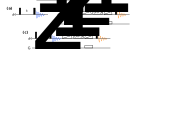
\includegraphics[]{pp/ct_states.png}%
    {\phantomsubcaption\label{fig:ct_states_c}}%
    {\phantomsubcaption\label{fig:ct_states_t}}%
    {\phantomsubcaption\label{fig:ct_states_ct}}%
    \caption[COSY/TOCSY NOAH module]{
        \textbf{(\subref*{fig:ct_states_c})} COSY module.
        \textbf{(\subref*{fig:ct_states_t})} TOCSY module; zero-quantum suppression is employed before and after the isotropic mixing period.
        \textbf{(\subref*{fig:ct_states_ct})} Combined COSY/TOCSY module, where the COSY FID is acquired immediately before the TOCSY mixing.
    }
    \label{fig:ct_states}
\end{figure}

As shown in entry 2 of \cref{tbl:noah_sensitivities}, this nesting of the COSY module does not materially affect the TOCSY sensitivity.
A small loss of approximately 20\% is observed, which is partly due to the imperfect magnetisation preservation by the HSQC, and perhaps also due to relaxation during the COSY acquisition period.
As for the time-saving factor, a slightly larger deviation ($\rho_t = 2.60$) is observed from the ideal value of $3$.
This reflects the addition of an extra acquisition period and the TOCSY mixing period, which make the assumption in \cref{eq:d1_limit} less valid.

\subsubsection{\noah{B,S}: HMBC + HSQC}

As mentioned previously, the HMBC module shown in \cref{fig:noah_sb_po_b} is designed to retain \magn{C} magnetisation through the addition of the $zz$-filter.
This can be used in a subsequent HSQC module in a \noah{B,S} supersequence.
Entry 3 of \cref{tbl:noah_sensitivities} shows that the addition of the $zz$-filter to the HMBC causes a relatively small 7\% decrease in sensitivity; on the other hand, the HSQC loses 13\% of its sensitivity because of incomplete magnetisation preservation.
These sensitivity losses, however, are reasonably acceptable considering the time savings provided by this supersequence ($\rho_t = 1.82$).

Generally, it has been recommended that less sensitive modules are placed earlier in the supersequence so that they can access a larger proportion of the equilibrium magnetisation.
The \noah{B,S} does not, however, actually obey this principle.
Since the HMBC is the less sensitive of the two modules, this rule of thumb suggests that the BS supersequence should be better than the alternative SB supersequence.
In fact, the opposite is true, as entry 4 of \cref{tbl:noah_sensitivities} shows.
This can be understood as follows: the HSQC module experiences a boost in sensitivity because it is placed first in the supersequence, and no longer needs to rely on the \magn{C} magnetisation preserved by the HMBC; and the HMBC benefits because the $zz$-filter modification is no longer needed.%
\footnote{In fact, the final \ang{180} pulse in the HMBC module could also be removed: this is likely to give a further boost in SNR, as discussed in \cref{subsec:noah__hmbc}. However, this was not done here.}
This may just be the exception that proves the rule, but in my view, this provides some justification for considering the ordering of modules on a case-by-case basis.

\subsubsection{\noah{B,S,C,T}: HMBC + HSQC + COSY + TOCSY}

We now move on to a longer supersequence containing four modules, with a correspondingly larger $\rho_t$ value of 3.22.
The sensitivity of the HSQC module is practically the same as in the \noah{B,S} supersequence just described: however, the COSY and TOCSY modules expose one weakness of the HMBC module which has so far been overlooked.
In principle, the HMBC module should only excite magnetisation of protons which have long-range couplings to \carbon{} (which we could, for example, denote as \magn{C(LR)}).
This magnetisation pool is distinct from both the directly coupled protons (\magn{C}), as well as protons which are not coupled to any \carbon{} at all (\magnnot{C}).
Unfortunately, this is not the case: it is not actually possible to separate the \magn{C(LR)} and \magnnot{C} magnetisation pools.
The HMBC excites both of these magnetisation sources, dephases the latter using CTP gradients, and detects the signal arising from the former.

This means that the COSY and TOCSY modules, which rely on \magnnot{C} magnetisation, will have substantially lower sensitivities.
The signal detected in these two modules derives only from polarisation that has recovered during the previous two acquisition periods, as shown in entry 5 of \cref{tbl:noah_sensitivities} (the values of $A$ for the COSY and TOCSY are 0.36 and 0.28 respectively).
That said, this is in fact not likely to be an issue \textit{even} for sensitivity-limited samples.
Because the intrinsic sensitivity of the HMBC is orders of magnitude lower than that of the COSY and TOCSY, the COSY and TOCSY spectra still have greater intensities than the HMBC, even after these large losses in sensitivity.
Thus, as long as the entire supersequence is acquired with enough scans such that the HMBC SNR is sufficient, the COSY and TOCSY will \textit{also} have acceptable SNR.
This is proven by the spectra shown in \cref{fig:bsct}.

A rather more insidious problem is that different signals relax at different rates: thus, the COSY and TOCSY spectra (or indeed, any homonuclear module) will have uneven intensities and are frequently asymmetric.
This can be seen in the COSY spectrum, where a pair of asymmetric crosspeaks are highlighted.
Adding a period of isotropic mixing before the COSY module\autocite{Kupce2018CC} can ameliorate this to some extent (although the spectra in \cref{fig:bsct} were not acquired with this).

\begin{figure}[!ht]
    \centering
    \includegraphics[]{noah/bsct.png}%
    {\phantomsubcaption\label{fig:bsct_b}}%
    {\phantomsubcaption\label{fig:bsct_s}}%
    {\phantomsubcaption\label{fig:bsct_c}}%
    {\phantomsubcaption\label{fig:bsct_t}}%
    \caption[Spectra obtained from a \noah{B,S,C,T} supersequence.]{
        Spectra obtained from a \noah{B,S,C,T} supersequence. 
        \textbf{(\subref*{fig:bsct_b})} HMBC.
        \textbf{(\subref*{fig:bsct_s})} HSQC.
        \textbf{(\subref*{fig:bsct_c})} COSY; a pair of crosspeaks with asymmetric intensities is highlighted with black arrows.
        \textbf{(\subref*{fig:bsct_t})} TOCSY (\qty{60}{\ms} DIPSI-2 mixing).
        Despite the COSY and TOCSY having only around 30\% of their sensitivity compared to standalone experiments, the intensity of the spectra obtained is still perfectly acceptable (the contour levels chosen are 1--2 orders of magnitude larger than for the HMBC).
        \datacode{7Z-220224}
    }
    \label{fig:bsct}
\end{figure}


\subsubsection{\noah{B,Spn,S,C,T}: HMBC + \nitrogen{} seHSQC + HSQC + COSY + TOCSY}

As the final example, we add a further magnetisation pool to the mix, namely protons directly coupled to \nitrogen{} (i.e.\ \magn{N}).
As of the time of writing, the implementation of multiple-FID experiments on Bruker spectrometers limits $N$ to a maximum of 5, so a supersequence such as this \noah{B,Spn,S,C,T} is the current limit.
(However, there is no \textit{scientific} argument forbidding $N > 5$, and it is likely that in future versions of TopSpin this restriction will be lifted.)

The values of $A$ for each module are given in entry 6 of \cref{tbl:noah_sensitivities}.
If the HMBC module is placed at the beginning of the supersequence, then in order to preserve \textit{both} \magn{N} and \magn{C} magnetisation, the $zz$-filter must be extended to include \nitrogen{} pulses\autocite{Kupce2019JMR}.
As before, this modification leads to a slight drop in sensitivity for the HMBC ($5\%$).

After this, the \nitrogen{} seHSQC and \carbon{} HSQC modules both suffer drops in sensitivity.
For the \nitrogen{} seHSQC, this is partly because of imperfect preservation of \magn{N} magnetisation by the HMBC, but also stems from the addition of the $zz$ isotope-selective pulse (ZIP) element to the seHSQC pulse sequence; this is described further in \cref{subsec:noah__sehsqc_n}.
On the other hand, for the \carbon{} HSQC, the sensitivity loss stems purely from imperfect retention of \magn{C} magnetisation by the HMBC.
Finally, because the HMBC dephases \magn{!X} magnetisation, the COSY and TOCSY at the end have lower sensitivities: however, as discussed above, this is not an issue in practice.

It is also possible to move the \nitrogen{} seHSQC module to the front: this gives it a slightly greater sensitivity, at the cost of the HMBC (entry 7, \cref{tbl:noah_sensitivities}).
In general, these two modules tend to have comparable sensitivity, and which of these two arrangements is better depends on which module the sensitivity needs to be optimised for.

Finally, the value of $\rho_t$ given here of 3.74 represents an effective upper limit on the time-saving factor.
Although $\rho_t$ increases with $N$, the extent to which it deviates from the ideal value of $N$ also increases: it is very difficult to obtain $\rho_t > 4$, even with five modules in the supersequence.
Of course, it is possible to increase $\rho_t$ further by lengthening the recovery delay $d_1$ used for the experiments: for example, if $d_1$ is increased to \qty{2}{\s} from its present value of \qty{1.5}{\s}, $\rho_t$ increases to 3.94.
Obviously, this can only be pushed so far before it becomes meaningless.


\section{GENESIS: automated pulse programme creation}
\label{sec:noah__genesis}

In this section, I discuss the development of the GENESIS (GENEration of Supersequences In Silico) website (\cref{fig:genesis_frontpage}): as the name suggests, it automatically generates pulse programmes for arbitrary NOAH supersequences.
The website also provides extensive instructions on acquiring and processing NOAH data.
Although this may at first glance appear slightly out of chronological order, in that the paper\autocite{Yong2022AC} was published later than much of the other work in this chapter, an early version of the GENESIS tool was in fact created much earlier (by July 2020).

The present version of GENESIS is available at \url{https://nmr-genesis.co.uk}.

\begin{figure}[!ht]
    \centering
    \includegraphics[draft=false,width=0.9\textwidth]{noah/genesis_frontpage.png}%
    \caption[Front page of the GENESIS website]{
        The front page of the GENESIS website (\url{https://nmr-genesis.co.uk}), as of 10 September 2022.
    }
    \label{fig:genesis_frontpage}
\end{figure}

\subsection{Motivation}
\label{subsec:noah__genesis_motivation}

From the preceding discussion in \cref{sec:noah__introduction}, it is clear that modules which use different magnetisation pools can be combined almost at will.
It does not matter \textit{what} modules they are, merely what magnetisation pools they consume (and preserve).
Thus, for example, the \noah{S,C} supersequence can in fact be generalised to any \magn{C} module plus any \magnnot{C} module.

Very broadly speaking, we may define a generic supersequence as having any or all of the following:

\begin{itemize}
    \item a HMBC module, which actually uses \magn{!X} magnetisation but can be placed at the front as discussed in the \noah{B,S,C} example above;
    \item a \magn{N} module;
    \item one or more \magn{C} modules (it is possible to partition the \magn{C} magnetisation pool between two modules, as will be discussed in \cref{subsec:noah__hsqctocsy});
    \item one or more \magn{!X} modules which consume bulk magnetisation.
\end{itemize}

In the first NOAH paper in 2017\autocite{Kupce2017ACIE}, a total of 285 `viable' supersequences were already listed.
If we further take into account some of the new modules which were developed over the course of my DPhil (\cref{sec:noah__modules}), this generic structure means that there are over 4000 viable supersequences.%
\footnote{This is also ignoring the `parallel' supersequences, which are discussed in \cref{sec:noah__parallel}. The support for parallel supersequences in GENESIS is not complete: integrating these fully would require substantial changes to the user interface, which I have not had time to do.}
(`Non-viable' sequences would be those which have undesirable drawbacks: for example, wrongly ordered modules like in a \noah{C,S} supersequence.)

Despite this, \textit{only around 45 pulse programmes} have been published in \textit{all} the NOAH papers to date, or submitted to the Bruker User Library.
Traditionally, NOAH pulse programmes must be written by hand, which is a laborious and fairly error-prone process made worse by the sheer length of these experiments.
Doing this for thousands of supersequence is clearly impractical; furthermore, each time a new module is developed, or an old module is improved, updating every relevant supersequence would itself already be a mammoth task.
This explains why---although the NOAH concept provides a clear blueprint for how supersequences may be constructed---there is still a huge gap between theory and practice.

To bridge this gap, I turned towards the \textit{programmatic} generation of pulse programmes.%
\footnote{This is actually a bit of a lie: GENESIS was initially created for my own convenience. Throughout this chapter, I have had to perform many comparisons of different supersequences, and this tool spared me from having to write everything by hand (and---more often than not---subsequently discover mistakes which invalidated the results). Of course, it soon became apparent that this could be much more widely applicable.}
This not only allows for existing supersequences to be generated at will, but also provides an easy way for updates to be rapidly disseminated to the NMR community.
Furthermore, a website can serve as a `one-stop' shop where---after downloading pulse programmes---users may download the associated NOAH processing scripts and also access instructions on how to run NOAH experiments.
This information did already exist, but was scattered across several different websites and/or journal supplementary information documents, and would have been needlessly confusing to a new user (not to mention the different versions of scripts available in different publications).


\subsection{Implementation details}
\label{subsec:noah__genesis_implementation}

I will now describe a few features of GENESIS pulse programmes, as well as how these are implemented.
The GENESIS code is written in TypeScript; during deployment, this is compiled to JavaScript, which can then be directly executed in the client's web browser.
No server-side code is required, meaning that the GENESIS web page is actually a static site (it is currently hosted using GitHub Pages).

\subsubsection{Overview}

The algorithm used for pulse programme construction can loosely be separated into three parts:
\begin{enumerate}
    \item the \textit{preamble}, which consists of everything up until the beginning of the actual pulse sequence (the \texttt{ze} command). This includes header comments (for the user) as well as definitions of parameters, such as delays and pulse widths;
    \item the \textit{main section}, which contains the actual pulse sequence;
    \item the \textit{epilogue}, which contains phase cycle information as well as footer comments describing each parameter. Instructions for generating shaped pulses using Bruker's WaveMaker software are also included here.
\end{enumerate}

\todo{FIG - breakdown of pulse sequence}

The construction of the preamble and main section is largely accomplished through the collation of module-specific information, the most important of which are:
\begin{itemize}
    \item information about the module itself, which go into the header comments;
    \item parameter definitions, which are collated to form the preamble. Duplicates must be removed here to avoid errors; and
    \item the pulse programmes themselves, which are directly concatenated to form the main section.
\end{itemize}
These, as well as other smaller bits of information (e.g.\ relevant citations, appropriate processing scripts), are stored within \texttt{NOAHModule} objects.
Each distinct module corresponds to one such object.
Therefore, if one wants to add a new module to GENESIS, most of the work can be completed by simply defining a new \texttt{NOAHModule} object: no changes to the algorithm itself are needed.%
\footnote{The website layout must also be changed so that users can actually select the new module.}

Since NOAH experiments are 2D experiments, there is one additional complication: the pulse programme must contain appropriate looping statements, together with pulse phase and delay incrementation, in order to correctly generate the indirect dimension.
In many existing NOAH pulse programmes, looping in 2D experiments was written using the equivalent of \texttt{for} loops (\todo{listing}).
Although this suffices for the vast majority of supersequences, the implementation of parallel supersequences was particularly problematic, as an additional nested loop must be added.
Thus, I opted to only use \textit{one} loop, and to control the phase and delay incrementation using modular arithmetic: the outcome is entirely equivalent, but there is no need to adjust the loop statement itself when switching between linear and parallel supersequences.

\todo{listings to illustrate the above}

To put the epilogue together, the pulse programme constructed so far is scanned for pulse phases, shaped pulses, and all other parameters.
Using predefined lookup tables, GENESIS then outputs pulse phase definitions, WaveMaker directives (where appropriate), and comments containing textual descriptions of each parameter.
These comments are mostly cosmetic, but are very useful to the user as they are displayed in the \texttt{ased} screen when setting up an experiment.
Finally, instructions for automatic processing of the NOAH data (explained in \cref{subsec:noah__genesis_motivation}) are added to the bottom, together with the version number and a timestamp (for reproducibility purposes).

\subsubsection{Module choice}

Developer mode

\subsubsection{Parameter standardisation}
\subsubsection{Parameter descriptions}
\subsubsection{Tests}
\subsubsection{How smart is GENESIS?}



\subsection{Processing improvements}
\label{subsec:noah__genesis_processing}

\section{Discussion of individual modules}
\label{sec:noah__modules}

\subsection{Sensitivity-enhanced HSQC}
\label{subsec:noah__sehsqc}

\carbon{} seHSQC

\nitrogen{} seHSQC

\subsection{HSQC-TOCSY}
\label{subsec:noah__hsqctocsy}

Having completed our survey of \nitrogen{} modules, we now return to \carbon{} modules: in particular, I was particularly interested in how \textit{two} (or more) modules drawing on \magn{C} magnetisation could be combined in the same supersequence.
Of course, this can be crudely accomplished by simply concatenating two modules which consume all \magn{C} magnetisation: the second of these modules will have greatly reduced sensitivity.
This is acceptable if the second module has a far greater intrinsic sensitivity, but this is not often the case with heteronuclear experiments: thus, a method of \textit{balancing} the sensitivities of the two modules is desirable.
Equivalently, we would like a way to \textit{partition} the magnetisation pool between multiple different modules as we see fit.


\subsubsection{Two HSQC modules}

The strategy used here is in fact a feature of the ASAP-HSQC experiment\autocite{SchulzeSunninghausen2014JACS,SchulzeSunninghausen2017JMR}, previously described in \cref{subsec:poise__asaphsqc}.
In this experiment (which also doubles up as the NOAH HSQC module), the INEPT delay $\DeltaE$ can be changed from its usual value of $1 / (4J)$ (where $J$ is short for $\oneJ{CH}$).
After the \ang{90}($I$)--$\DeltaE$--\ang{180}($I,S$)--$\DeltaE$ INEPT block, the relevant product operators are
\begin{equation}
    \label{eq:inept_changed}
    \cos(2\pi J\DeltaE) I_y - \sin(2\pi J\DeltaE) 2I_xS_z.
\end{equation}
In a `normal' INEPT block, the choice of $\DeltaE = 1/(4J)$ makes the cosine term vanish, leaving us with only the term $-2I_xS_z$.
Since this term is subsequently transferred to spin $S\/$ and labelled in $t_1$, this corresponds to \textit{complete} excitation of \magn{C} magnetisation.

However, if we choose $\DeltaE < 1/(4J)$, then the first $I_y$ term can be `stored' as unexcited \magn{C} magnetisation;
if the remainder of the sequence returns \textit{this} to the $+z$ state, then this portion can be used in a second experiment.
Indeed, this is what happens in the ASAP-HSQC experiment (i.e.\ NOAH HSQC module).
Thus, we could simply construct a \noah{S,S,C} experiment in which the first HSQC module has a suitably modified value of $\DeltaE$: this would achieve the stated aim of partitioning \magn{C} magnetisation between two different modules.
Specifically, in order to excite a fraction $f\/$ of \magn{C} magnetisation (and store the remaining $(1 - f)$ for the next module), we require that
\begin{equation}
    \label{eq:ssc_inept_delay}
    \DeltaE = \frac{2\Delta \arcsin f}{\pi}
\end{equation}
where $\Delta$ is the usual value of $1/(4J)$.
The resulting spectra, obtained by setting $f = 0.8$, are shown in \cref{fig:sscc_example}.


\begin{figure}[!ht]
    \centering
    \includegraphics[draft=false]{noah/sscc_example.png}%
    {\phantomsubcaption\label{fig:sscc_example_s1}}%
    {\phantomsubcaption\label{fig:sscc_example_s2}}%
    {\phantomsubcaption\label{fig:sscc_example_cc}}%
    \caption[Spectra from \noah{S,S,Cc} supersequence]{
        Spectra from a \noah{S,S,Cc} supersequence, where the INEPT delay of the first HSQC module was modified to only excite a fraction $f = 0.7$ of \magn{C} magnetisation.
        \textbf{(\subref*{fig:sscc_example_s1})} First HSQC.
        \textbf{(\subref*{fig:sscc_example_s2})} Second HSQC.
        \textbf{(\subref*{fig:sscc_example_cc})} CLIP-COSY.
        \datacode{7A-201010}
    }
    \label{fig:sscc_example}
\end{figure}

In \cref{fig:sscc_improvements_base}, the intensities of these spectra are compared against the HSQC and CLIP-COSY in a \noah{S,Cc} supersequence.
As expected, the first HSQC has 80\% of its sensitivity.
However, the second HSQC spectrum has around 65\% of this `base' sensitivity, despite only nominally having 20\% of the \magn{C} magnetisation to work with.
This is largely due to \magn{C} magnetisation which recovers during the FID of the first HSQC.
Since both HSQC modules do not perfectly preserve \magnnot{C} magnetisation, the CLIP-COSY experiences a very small sensitivity loss (compared to a \noah{S,Cc} supersequence where only one HSQC module is used, which in turn is slightly less sensitive than a standalone CLIP-COSY).

\begin{figure}[!ht]
    \centering
    \includegraphics[draft=false]{noah/sscc_improvements.png}%
    {\phantomsubcaption\label{fig:sscc_improvements_base}}%
    {\phantomsubcaption\label{fig:sscc_improvements_sehsqc}}%
    {\phantomsubcaption\label{fig:sscc_improvements_dipsi}}%
    {\phantomsubcaption\label{fig:sscc_improvements_mfa}}%
    \caption[Sensitivity comparisons for \noah{S,S,Cc} and \noah{S,Sp,Cc} supersequences]{
        Comparisons of HSQC and CLIP-COSY sensitivities of \noah{S,S,Cc} and \noah*{S,Sp,Cc} supersequences.
        The fraction of \magn{C} magnetisation excited in the first module, $f$, is set to $0.8$.
        Peak intensities are normalised against the HSQC and CLIP-COSY experiments in a \noah{S,Cc} supersequence.
        \textbf{(\subref*{fig:sscc_improvements_base})} \noah{S,S,Cc} (the same spectra as shown in \cref{fig:sscc_example}).
        \textbf{(\subref*{fig:sscc_improvements_sehsqc})} \noah{S,Sp,Cc}.
        \textbf{(\subref*{fig:sscc_improvements_dipsi})} \noah{S,S,Cc} with \qty{35}{\ms} DIPSI-2 mixing after the first HSQC module.
        \textbf{(\subref*{fig:sscc_improvements_mfa})} A \noah{S,S,Cc} supersequence, but using the seHSQC-splitting implementation of Nolis et al.\autocite{Nolis2019CPC} (as opposed to the ASAP-HSQC module) for the double HSQC.
    }
    \label{fig:sscc_improvements}
\end{figure}

The sensitivity of the second HSQC module can be further improved by simply using the seHSQC module (specifically, the seHSQC2) in place of it.
The effects of this are shown in \cref{fig:sscc_improvements_sehsqc}: sensitivity improvements are obtained in that module itself (although they are not uniform as they depend on multiplicity), and the CLIP-COSY sensitivity is decreased slightly due to poorer \magnnot{C} preservation.
These are entirely in line with the previous discussion in \cref{subsec:noah__sehsqc_c}.

It is also possible to include a period of isotropic mixing between the two HSQC modules: here, the DIPSI-2 sequence\autocite{Shaka1988JMR} was chosen.
Since the \magn{C} magnetisation pool has been (partially) depleted, and the \magnnot{C} magnetisation pool is (almost) full, this should in theory lead to transfer of polarisation from the \magnnot{C} pool to \magn{C}.
However, when tested, this was not found to have a beneficial impact on the supersequence sensitivity (\cref{fig:sscc_improvements_dipsi}): in fact, 
One caveat is that this leads to slightly uneven intensities: since DIPSI transfers magnetisation through scalar couplings, peaks corresponding to protons with fewer coupling partners experience smaller gains in intensity.

\todo{Pulse sequence with prod ops??}

\todo{Multiplicity editing --- not properly implemented in GENESIS?!}


On its own, the acquisition of two HSQC spectra---as has so far been shown---is not particularly interesting.
However, it is possible to differentiate the two HSQC signals and thereby extract more information.
For example, one spectrum may be run without decoupling in order to measure one-bond coupling constants\autocite{Enthart2008JMR,Nolis2019CPC}; or the indirect-dimension spectral width of one of the HSQC spectra can be changed in order to make use of spectral aliasing techniques\autocite{Nolis2019JMR,Jeannerat2011eMR}.
The pulse sequence itself may also be modified: for example, the addition of an isotropic mixing block to the first HSQC yields a HSQC-TOCSY + HSQC combination\autocite{Nolis2019CPC}, which I now discuss.


\subsubsection{HSQC-TOCSY}

The addition of DIPSI mixing
This in fact leads to the ASAP-HSQC-TOCSY experiment, also previously reported by Luy and coworkers\autocite{Becker2019JMR}.


\subsection{HSQC-COSY}
\label{subsec:noah__hsqc_cosy}

Blah.

\subsection{2DJ and PSYCHE}
\label{subsec:noah__2djpsyche}

So far, I have exclusively used the CLIP-COSY as the final homonuclear module in NOAH supersequences.
In general, since homonuclear modules are placed at the end of supersequences, there is rarely any need to adapt them for NOAH supersequences, as they do not need to preserve any magnetisation.
One exception to this is the family of 2DJ and pseudo-2D pure shift experiments (here typified by PSYCHE), where the spectral width in the indirect dimension is extremely small, on the order of \qty{50}{\Hz}.
In such cases, the number of $t_1$ increments required is far smaller than for a typical 2D experiment.
Since---by default---each module in a NOAH supersequence is acquired with the same number of increments, directly concatenating such modules to the end of a supersequence would therefore prove suboptimal.

However, as described previously in \cref{subsec:noah__hmqc,subsec:noah__sehsqc_n}, it is possible to reduce the number of $t_1$ increments for a particular module, and in exchange, increase the number of scans recorded for that module.
In the context of \nitrogen{} modules, this was a `special' procedure referred to as $k$-scaling; however, for these homonuclear modules, it is natural and necessary.
One difference in the implementation is that, instead of specifying a value $k$ by which \texttt{TD1} is scaled down and \texttt{NS} scaled up, the user is allowed to directly specify the number of $t_1$ increments as an integer (\texttt{CNST37} in TopSpin).
This value must be a divisor of the \textit{normal} number of $t_1$ increments for all other modules (or equivalently, in the context of \nitrogen{} modules, $k$ must be an integer).
The `indirect-dimension spectral width' is specified as \texttt{CNST38}: this quantity is more properly referred to as the reciprocal of the chunk size, i.e.\ $1/\Tchunk$.

\begin{figure}[!ht]
    \centering
    \includegraphics[]{noah/2dj_example.png}%
    {\phantomsubcaption\label{fig:2dj_example_spn}}%
    {\phantomsubcaption\label{fig:2dj_example_spc}}%
    {\phantomsubcaption\label{fig:2dj_example_j}}%
    \caption[Spectra from a \noah{Spn,Sp,J} supersequence]{
        Spectra obtained from a \noah{Spn,Sp,J} supersequence.
        \textbf{(\subref*{fig:2dj_example_spn})} \nitrogen{} seHSQC (256 $t_1$ increments and 2 scans per increment).
        \textbf{(\subref*{fig:2dj_example_spc})} \carbon{} seHSQC.
        \textbf{(\subref*{fig:2dj_example_j})} PSYCHE 2DJ (32 $t_1$ increments and 8 scans per increment).
        \datacode{7G-201028}
    }
    \label{fig:2dj_example}
\end{figure}

The modules thus implemented include the standard magnitude-mode 2DJ experiment, the PSYCHE 2DJ experiment\autocite{Foroozandeh2015CC}, the original 1D PSYCHE\autocite{Foroozandeh2014ACIE}, and the 1D TSE-PSYCHE\autocite{Foroozandeh2015CC}.
An example of the data thus obtained (with the PSYCHE 2DJ) is shown in \cref{fig:2dj_example}.
One particular advantage of including PSYCHE-type modules in NOAH supersequences is that sensitivity is not likely to be at a premium: this is partly because of the increased number of scans, but also partly because other 2D experiments have comparably low sensitivity (meaning that in the time needed to acquire an HSQC, for example, the PSYCHE experiment will also have sufficient sensitivity).
This allows the user to choose a relatively small flip angle (ca.\ \ang{10}) for the PSYCHE saltire pulses in order to minimise artefacts from imperfect decoupling (see also \cref{subsec:pureshift__psyche_analysis}).

\begin{figure}[!ht]
    \centering
    \includegraphics[]{noah/psyche_wrongsw1.png}%
    {\phantomsubcaption\label{fig:psyche_wrongsw1_bad_nosap}}%
    {\phantomsubcaption\label{fig:psyche_wrongsw1_bad_sap}}%
    {\phantomsubcaption\label{fig:psyche_wrongsw1_good_nosap}}%
    {\phantomsubcaption\label{fig:psyche_wrongsw1_good_sap}}%
    {\phantomsubcaption\label{fig:psyche_wrongsw1_good_nosap_25}}%
    {\phantomsubcaption\label{fig:psyche_wrongsw1_good_sap_25}}%
    \caption[Effect of automatic chunk size calculation and SAPPHIRE averaging on NOAH PSYCHE spectra]{
        A series of 1D PSYCHE spectra obtained from the \noah{Spn,Sp,P} supersequence (saltire flip angle of \ang{15}).
        \textbf{(\subref*{fig:psyche_wrongsw1_bad_nosap})} 1D PSYCHE spectrum acquired without SAPPHIRE averaging, and an incorrect chunk size which is not an integral number of complex data points. The `indirect-dimension spectral width' (more precisely, $1/\Tchunk$) is \qty{50}{\Hz}.
        \textbf{(\subref*{fig:psyche_wrongsw1_bad_sap})} 1D PSYCHE spectrum with  8-step SAPPHIRE averaging and an incorrect chunk size; this manifests as phase errors which cannot be corrected.
        \textbf{(\subref*{fig:psyche_wrongsw1_good_nosap})--(\subref*{fig:psyche_wrongsw1_good_sap})} The same as (\subref*{fig:psyche_wrongsw1_bad_nosap}) and (\subref*{fig:psyche_wrongsw1_bad_sap}), but with the chunk size automatically corrected in the pulse programme.
        \textbf{(\subref*{fig:psyche_wrongsw1_good_nosap_25})--(\subref*{fig:psyche_wrongsw1_good_sap_25})} The same as (\subref*{fig:psyche_wrongsw1_good_nosap}) and (\subref*{fig:psyche_wrongsw1_good_sap}), but with double the chunk size.
        This leads to a more striking difference between the data acquired without and with SAPPHIRE, as discussed in the original paper\autocite{Moutzouri2017CC}.
        \datacode{7C-211123}
    }
    \label{fig:psyche_wrongsw1}
\end{figure}

On top of this, for the 1D (TSE-)PSYCHE sequences, the extra transients can be used to perform SAPPHIRE averaging\autocite{Moutzouri2017CC}.
Ordinarily, the PSYCHE pulse sequence seeks to refocus J-couplings in the middle of each chunk (of duration $\Tchunk$).
This is accomplished through the \textit{prefocusing} of J-couplings in a spin echo of total duration $\Tchunk/2$.\autocite{Aguilar2010ACIE}
In the SAPPHIRE procedure, each chunk of the pure shift interferogram is instead collected several times, all while varying the exact point in time where J-coupling is perfectly refocused.
Summation of these data leads to the suppression of artefacts which arise due to the periodic J-modulation in the interferogram.
This averaging is somewhat analogous to a phase cycle, and performing an 8-step SAPPHIRE averaging procedure (for example) would often require the experiment to be lengthened beyond the duration which is truly necessary.
However, in the context of NOAH, since each chunk is acquired at least $k$ times, a $k$-step SAPPHIRE procedure can be performed `for free'.
In the GENESIS pulse programmes, this feature is enabled by default, although it can be turned off by selecting the original modules using developer mode.

A final and more prosaic implementation detail is that in the 1D pure shift modules, the chunk size $\Tchunk$ is automatically rounded to the nearest even multiple of the dwell time $\tau_{\symup{dw}}$ (\texttt{DW} in TopSpin).
This ensures that each chunk consists of an integral number of complex data points.
Although this can be set by the user manually, it is very easy to forget, especially for someone not fully acquainted with the experiment; the results can be quite different, as illustrated in \cref{fig:psyche_wrongsw1}.
When an $n$-step SAPPHIRE averaging is used, the requirement is even stricter: $\Tchunk$ must be a multiple of $2n \tau_{\symup{dw}}$.
This is also encoded in the pulse programmes.

\subsection{DQF-COSY}
\label{subsec:noah__dqf_cosy}

States vs EA

\subsection{\texorpdfstring{\nitrogen{}}{15N} HMQC}
\label{subsec:noah__hmqc}

In \cref{subsec:noah__sehsqc_n}, I will discuss how the sensitivity-enhanced HSQC modules developed above may be adapted into \proton{}--\nitrogen{} experiments.
However, before that, I make a slight detour to cover the \nitrogen{} HMQC experiment, which (up until my DPhil) was the experiment of choice for detecting one-bond \proton{}--\nitrogen{} correlations.

\begin{figure}[htb]
    \centering
    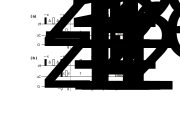
\includegraphics[draft=false]{pp/hmqc/all.png}%
    {\phantomsubcaption\label{fig:noah_hmqc_2grad}}%
    {\phantomsubcaption\label{fig:noah_hmqc_4grad}}%
    \caption[NOAH HMQC pulse sequences]{
        \textbf{(\subref{fig:noah_hmqc_2grad})} With two encoding gradients around $t_1$.
        \textbf{(\subref{fig:noah_hmqc_4grad})} With four encoding gradients around $t_1$.
        Phase cycling is performed with $\phi_1 = (x, -x)$, $\phi_2 = (x, x, -x, -x)$, and $\phi_\text{rec} = (x, -x, -x, x)$.
        The delay $\Delta$ is set to $1 / (4 \cdot \oneJ{NH})$.
        Gradient amplitudes are: $g_1 = 80\%$; $g_2 = \pm 32.4\%$; $g_2' = g_2/2$.
    }
    \label{fig:noah_hmqc}
\end{figure}

The HMQC module is based on the ASAP-HMQC reported by Kup{\v{c}}e and Freeman\autocite{Kupce2007MRC}, which used a symmetric gradient scheme similar to that in the seHSQC modules previously described (\cref{fig:noah_hmqc_2grad}).
However, in the NOAH module\autocite{Kupce2017ACIE}, bipolar gradient pulse pairs were placed before and after $t_1$ (\cref{fig:noah_hmqc_4grad}).
This was likely implemented in order to allow the final gradient, $g_2$, to have as large an amplitude as possible.
In heteronuclear experiments, this final gradient is particularly important for dephasing bulk magnetisation which is transverse just prior to detection (due to pulse imperfections or relaxation).
If this gradient is too weak, this unwanted magnetisation will be incompletely dephased, leading to artefacts in the resulting spectrum.

Strategies to maximise this gradient amplitude are particularly crucial in \proton{}--\nitrogen{} experiments (as compared to \proton{}--\carbon{} experiments) for two reasons.
Firstly, the natural abundance of \nitrogen{} (0.36\%) is even smaller than \carbon{} (1.1\%), meaning that better suppression must be achieved in order for the artefacts to not obscure the signal.
Secondly, the gyromagnetic ratio of \nitrogen{} is also smaller: thus, since $g_2/g_1 \propto \gammaN/\gammaH$, an unmodified pulse sequence will naturally have a smaller $g_2$.

In this respect, the four-gradient scheme in \cref{fig:noah_hmqc_4grad} is superior to the two-gradient scheme, because the gradient $g_2$ will have an amplitude of $4\gammaN g_1/\gammaH$.
However, when used in a NOAH supersequence, this leads to wing artefacts in downstream modules, since bulk \magnnot{N} magnetisation effectively does not experience any coherence order selection during $t_1$.
This motivates a return to the two-gradient scheme of \cref{fig:noah_hmqc_2grad}.
To compensate for the fact that the decoding gradient $g_2'$ has half of the amplitude of $g_2$, all CTP gradients were instead \textit{lengthened} from their usual duration of \qty{1}{\ms} to \qty{2.5}{\ms}.
This ensures that any stray transverse bulk magnetisation at the end of the HMQC module is effectively dephased.

The HMQC spectra thus obtained are shown in \cref{fig:hmqc_grad_spec}.

\begin{figure}[!ht]
    \centering
    \includegraphics[draft=false]{noah/hmqc_grad.png}%
    {\phantomsubcaption\label{fig:hmqc_grad_spec_2grad_1ms_hmqc}}%
    {\phantomsubcaption\label{fig:hmqc_grad_spec_2grad_1ms_hmqcp}}%
    {\phantomsubcaption\label{fig:hmqc_grad_spec_2grad_1ms_cosy}}%
    {\phantomsubcaption\label{fig:hmqc_grad_spec_4grad_1ms_hmqc}}%
    {\phantomsubcaption\label{fig:hmqc_grad_spec_4grad_1ms_hmqcp}}%
    {\phantomsubcaption\label{fig:hmqc_grad_spec_4grad_1ms_cosy}}%
    {\phantomsubcaption\label{fig:hmqc_grad_spec_2grad_2p5ms_hmqc}}%
    {\phantomsubcaption\label{fig:hmqc_grad_spec_2grad_2p5ms_hmqcp}}%
    {\phantomsubcaption\label{fig:hmqc_grad_spec_2grad_2p5ms_cosy}}%
    \caption[Comparison of \noah{M,Sp,Cc} modules with different HMQC gradient schemes]{
        Comparison of HMQC and CLIP-COSY spectra obtained from \noah{M,Sp,Cc} supersequences, acquired using different HMQC gradient schemes.
        In the first row, the HMQC spectrum itself is shown.
        In the second row, the positive projection of the HMQC spectrum onto the $f_2$ axis is shown; the numbers indicate peak intensities with respect to the reference dataset (the left column).
        In the third row, (an inset of) the CLIP-COSY spectrum is shown.
        \textbf{(\subref{fig:hmqc_grad_spec_2grad_1ms_hmqc})--(\subref{fig:hmqc_grad_spec_2grad_1ms_cosy})} Using the two-gradient scheme of \cref{fig:noah_hmqc_2grad}, with \qty{1}{ms} gradients.
        \textbf{(\subref{fig:hmqc_grad_spec_4grad_1ms_hmqc})--(\subref{fig:hmqc_grad_spec_4grad_1ms_cosy})} Using the four-gradient scheme of \cref{fig:noah_hmqc_4grad}, with \qty{1}{ms} gradients.
        \textbf{(\subref{fig:hmqc_grad_spec_2grad_2p5ms_hmqc})--(\subref{fig:hmqc_grad_spec_2grad_2p5ms_cosy})} Using the two-gradient scheme of \cref{fig:noah_hmqc_2grad}, with \qty{2.5}{ms} gradients.
    }
    \label{fig:hmqc_grad_spec}
\end{figure}

\subsection{HMBC}
\label{subsec:noah__hmbc}

The HMBC module is one which in fact does not fit perfectly into the NOAH principle of only exciting magnetisation which is needed.
As described in \cref{subsec:noah__case_studies}, the HMBC module should only require magnetisation of protons which have long-range couplings to \carbon{}; however, it ends up exciting \textit{all} \magnnot{C} magnetisation.
This leads to sharply reduced, and also unbalanced, intensities of homonuclear modules which come later in the supersequences.

I made some early (and brief) attempts at devising a pulse sequence which sought to discriminate these two magnetisation components using a perfect echo\autocite{Parella2019MRC}.
However, this was quickly abandoned as it proved very difficult to \textit{also} retain \magn{C} magnetisation.
I do not claim here that it is impossible to come up with a pulse sequence which does this, but it is certainly not easy, and ultimately I turned my focus to improving (rather than replacing) the HMBC module.


\subsubsection{Suppression of one-bond artefacts}

One of the issues with the NOAH HMBC module was that there were an unusual amount of one-bond artefacts, which arise from \magn{C} magnetisation which is allowed to evolve during the pulse sequence.
Generally, HMBC experiments seek to suppress this through the use of a low-pass J-filter (LPJF, see also \cref{subsec:poise__hmbc}).
The NOAH HMBC module \textit{additionally} contains a $zz$-filter, which stores \magn{C} magnetisation along $+z$ before the LPJF.
Thus, in theory, one-bond artefacts should be suppressed in the NOAH HMBC to an even greater extent.

However, this expectation is not borne out: in some cases, the NOAH HMBC in fact has \textit{more intense} one-bond artefacts when compared against a standard HMBC experiment (\cref{fig:noah_hmbc_1jch_no90,fig:noah_hmbc_1jch_std_lp2}).
Even performing an optimisation of the LPJF delays, as described in \cref{subsec:poise__hmbc}, did not lead to any reduction in artefacts.
I hypothesised instead that these artefacts arose from imperfect manipulation of \magn{C} magnetisation by the $zz$-filter.%
\footnote{It would be nice to back this up with simulations, but I did not have the time to run these.}
In particular, any \textit{antiphase} magnetisation (of the form $I_xS_z$ or $I_yS_z$) generated after the $zz$-filter would be reconverted into in-phase $I_x$ or $I_y$ terms, which would not be destroyed by the LPJF.
(The LPJF works based on the assumption that there is in-phase magnetisation at the beginning of it, which is true if the excitation element is just a \proton{} \ang{90} pulse.)

Such antiphase terms can be easily removed by the addition of a \carbon{} \ang{90} pulse, which transforms them into a mixture of double- and zero-quantum terms: these are either unobservable, or can be efficiently dephased by CTP gradients.
This technique is used in the CLIP-HSQC family of experiments\autocite{Enthart2008JMR,Gyongyosi2021AC}, as well as the LPJF itself.
In this case, we simply need to add an additional \carbon{} \ang{90} pulse at the end of the $zz$-filter: this pulse is highlighted in \cref{fig:noah_sb_po_b}.
This results in a striking reduction of the one-bond artefacts, as shown in \cref{fig:noah_hmbc_1jch_90}.
The suppression accomplished with the addition of this \ang{90} pulse is superior to that in the standard HMBC (\cref{fig:noah_hmbc_1jch_std_lp2}), and is comparable to a standard HMBC with a third-order LPJF (\cref{fig:noah_hmbc_1jch_std_lp3}).
Of course, the NOAH module---which by default uses a second-order LPJF---can also be `upgraded' to use a third-order LPJF.
In GENESIS pulse programmes, this can be done using the \texttt{-DLP3} acquisition flag (although the results were not evaluated here).

\begin{figure}[!ht]
    \centering
    \includegraphics[]{noah/hmbc_1jch.png}%
    {\phantomsubcaption\label{fig:noah_hmbc_1jch_no90}}%
    {\phantomsubcaption\label{fig:noah_hmbc_1jch_90}}%
    {\phantomsubcaption\label{fig:noah_hmbc_1jch_std_lp2}}%
    {\phantomsubcaption\label{fig:noah_hmbc_1jch_std_lp3}}%
    \caption[Suppression of one-bond artefacts in NOAH HMBC spectra]{
        \textbf{(\subref*{fig:noah_hmbc_1jch_no90})} NOAH $zz$-HMBC module without the additional \ang{90} pulse.
        One-bond artefacts are highlighted in red.
        \textbf{(\subref*{fig:noah_hmbc_1jch_90})} NOAH $zz$-HMBC with the \ang{90} pulse.
        \textbf{(\subref*{fig:noah_hmbc_1jch_std_lp2})} Standard library HMBC with a second-order LPJF.
        \textbf{(\subref*{fig:noah_hmbc_1jch_std_lp3})} Standard library HMBC with a third-order LPJF.
        \datacode{7A-210916}
    }
    \label{fig:noah_hmbc_1jch}
\end{figure}


\subsubsection{Gradient selection schemes}

Another point which was investigated (but bore less fruit) was the gradient scheme used for CTP selection.
The NOAH module, as shown in \cref{fig:noah_sb_po_b}, uses a `symmetric' scheme where two gradients of equal amplitude surround the $t_1$ period: this encoding is later decoded by a third gradient just prior to acquisition.
However, other choices exist: for example, the Bruker standard library HMBC (derived from the work of Cicero et al.\autocite{Cicero2001JMR}) uses only two gradients in total, which have unequal amplitudes.

This gradient scheme cannot be directly used in a NOAH HMBC module, though.
This is because the $zz$-filter element places \magn{C} magnetisation along the $+z$ axis just before the HMBC J-evolution delay (see \cref{fig:noah_sb_po_b}).
This magnetisation later experiences the \proton{} \ang{180} pulse in the middle of $t_1$, which means that an extra \ang{180} pulse must be added at the very end of the sequence to finally return it to $+z$.
It is necessary to ensure that there is at least one gradient placed after this \ang{180} pulse to ensure proper CTP selection (in the `symmetric' scheme of \cref{fig:noah_sb_po_b}, this is fulfilled by the gradient $g_2$).

\begin{figure}[!htbp]
    \centering
    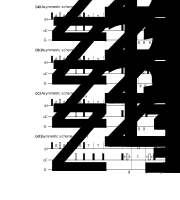
\includegraphics[]{pp/hmbc/noah_grads.png}%
    {\phantomsubcaption\label{fig:noah_hmbc_grads_bga}}%
    {\phantomsubcaption\label{fig:noah_hmbc_grads_bgb}}%
    {\phantomsubcaption\label{fig:noah_hmbc_grads_bgc}}%
    {\phantomsubcaption\label{fig:noah_hmbc_grads_b}}%
    \caption[Alternative CTP gradient schemes investigated for NOAH HMBC]{
        Alternative CTP gradient schemes investigated for the NOAH HMBC module.
        The coherences selected for during each gradient are indicated above each gradient, using the same notation for product operators as described in the \textit{Preface}: the `upper' term (e.g.\ $+$ in $\pm$) refers to the echo experiment, and the `lower' term to the antiecho experiment.
        So, for example, $+\pm$ refers to selection of $I_+S_+$ during the echo experiment and $I_+S_-$ during the antiecho experiment.
        Gradient amplitudes are as described in the text.
        \textbf{(\subref*{fig:noah_hmbc_grads_bga})} `Asymmetric scheme A', modified from the standard library sequence to include an additional \ang{180} pulse and gradient.
        \textbf{(\subref*{fig:noah_hmbc_grads_bgb})} `Asymmetric scheme B', where the \ang{180} pulse is shifted forward to the end of $t_1$.
        \textbf{(\subref*{fig:noah_hmbc_grads_bgc})} `Asymmetric scheme C', which modifies the $zz$-filter instead of using an extra \ang{180} pulse.
        \textbf{(\subref*{fig:noah_hmbc_grads_b})} The original `symmetric' scheme (the same as in \cref{fig:noah_sb_po_b}), placed here for convenience.
    }
    \label{fig:noah_hmbc_grads}
\end{figure}

Using this knowledge, it is possible to construct several `asymmetric' gradient schemes:
\begin{enumerate}
    \item `Scheme A' (\cref{fig:noah_hmbc_grads_bga}) is modified from the Bruker standard library to include a \ang{180} pulse and gradient at the end.
        The presence of an additional gradient means that there is a free parameter, here denoted as $\alpha$, which can be used to control the relative amplitudes of these three CTP gradients.
        The gradient amplitudes are chosen as follows:
        \begin{align}
            &\text{echo:}     & g_1 &= gc_1 & g_2 &= g    & g_3 &= gc_2 \label{eq:noah_hmbc_grads_bga_echo} \\
            &\text{antiecho:} & g_1 &= g    & g_2 &= gc_1 & g_3 &= gc_2 \label{eq:noah_hmbc_grads_bga_antiecho}
        \end{align}
        where $c_1 = -\alpha(\gammaH - \gammaC)/(\gammaH + \gammaC)$ and $c_2 = (1 - \alpha) (\gammaH - \gammaC)/\gammaH$.
        In principle $g$ is also a free parameter; for maximum suppression of artefacts I chose a relatively large value of 80\%.
    \item In `Scheme B' (\cref{fig:noah_hmbc_grads_bgb}), the \ang{180} pulse is shifted to immediately after $t_1$, before any of the CTP gradients have been applied. This means that there is no need for a third gradient, and the CTP gradient amplitudes can be directly taken from the standard library sequence:
        \begin{align}
            &\text{echo:}     & g_1 &= g  & g_2 &= gc \label{eq:noah_hmbc_grads_bgb_echo} \\
            &\text{antiecho:} & g_1 &= gc & g_2 &= g \label{eq:noah_hmbc_grads_bgb_antiecho}
        \end{align}
        where $c = -(\gammaH - \gammaC)/(\gammaH + \gammaC)$ and $g = 80\%$.
    \item `Scheme C' (\cref{fig:noah_hmbc_grads_bgc}) simply does not add a \ang{180} pulse, but instead modifies the phases of the $zz$-filter in order to place \magn{C} magnetisation along the $-z$ axis during the HMBC J-evolution delay.
        Here, the gradient amplitudes are the same as those in the standard library sequence as well as in scheme B.
\end{enumerate}

It is of interest to note two limiting cases of scheme A: when $\alpha = (\gammaH + \gammaC)/(\gammaH - \gammaC) \approx 1.67$, we have that $g_1 : g_2 : g_3 = 1 : -1 : \pm 2\gammaC/\gammaH$, which mimics the original `symmetric' scheme (\cref{fig:noah_hmbc_grads_b}); and when $\alpha = 1$, we have that $g_3 = 0$, i.e.\ a return to the two-gradient tactic of schemes B and C.
In the tests which follow, I ran scheme A with $\alpha = 1.67$, $\alpha = 0.6$, and $\alpha = 0.3$.

\begin{figure}[htb]
    \centering
    \includegraphics[]{noah/hmbc_grad_sens.png}%
    \caption[Comparison of relative sensitivities of HMBC gradient schemes]{
        Sensitivities of various asymmetric HMBC gradient schemes, as compared to the symmetric scheme in \cref{fig:noah_sb_po_b}.
        Each dot indicates one crosspeak in the HMBC spectrum; the numbers in parentheses are the average over all peaks.
        \datacode{7A-211226}
    }
    \label{fig:hmbc_grad_sens}
\end{figure}

All of the different HMBC versions above, plus the original `symmetric' scheme in \cref{fig:noah_sb_po_b}, were tested in the context of a \noah{B,S} supersequence using the andrographolide sample (\cref{fig:hmbc_grad_sens}).
Since the HMBC module is the first module in this supersequence, the values here are an accurate reflection of their intrinsic sensitivities.
As can be seen, there is not much at all which separates the different versions (outliers with $>2\times$ `sensitivity improvements' can be attributed to different J-modulation in the multiplet).
The most sensitive of these is asymmetric scheme C, which may be explained by the fact that it has one fewer \ang{180} pulse: however, this comes with an immediate drawback.
Since scheme C places the \magn{C} magnetisation along $-z$ during the LPJF as well as the J-evolution delay $\Delta_\text{LR}$ (a total of ca.\ \qty{70}{\ms}), relaxation losses during this period lead to poorer retention of \magn{C} magnetisation for later modules, as shown by the decreased HSQC sensitivities in \cref{fig:hmbc_grad_sens_hsqc}.
In contrast, all the other gradient schemes retain \magn{C} magnetisation equally well.

\begin{figure}[htb]
    \centering
    \includegraphics[]{noah/hmbc_grad_sens_hsqc.png}%
    \caption[Effect of HMBC gradient scheme on HSQC sensitivity in a \noah{B,S} supersequence]{
        Sensitivities of the HSQC module in a \noah{B,S} supersequence, where the HMBC module is implemented using the gradient schemes of \cref{fig:hmbc_grad_sens}.
        \datacode{7A-211226}
    }
    \label{fig:hmbc_grad_sens_hsqc}
\end{figure}

The final point worth studying is the quality of the HMBC spectrum itself.
To do this, we need to look at the actual spectra (\cref{fig:hmbc_grad_spec}).
For the most part, the spectra are all the same; however, there is a notable set of artefacts present in \cref{fig:hmbc_grad_spec_asymma1} (scheme A with $\alpha = 1.67$) as well as \cref{fig:hmbc_grad_spec_asymmb} (scheme B), highlighted in red boxes.
These artefacts occur at the frequencies
\begin{equation}
    \label{eq:hmbc_wing_artefacts}
    (\Omega_1, \Omega_2) = \left(\Omega_S \pm \frac{\Omega_I}{2}, \Omega_I\right),
\end{equation}
and are in fact `wing' artefacts similar to that observed in other modules (\cref{subsec:noah__sehsqc_c,subsec:noah__hmqc,subsec:noah__sehsqc_n}).
In this case, they arise due to imperfect refocusing of the \proton{} chemical shift during $t_1$: specifically, whenever $I_zS_\pm$ terms are present during the second half of $t_1$.
Extra evidence for the origin of these artefacts comes from the observation that when the \ang{180} pulse in the middle of $t_1$ is phase cycled, the artefacts are removed.
In a standard HMBC, these terms would not be detected in the final FID; however, in this case, the addition of an extra \ang{180} pulse after $t_1$ provides an opportunity for these to be converted back into observable spin-$I\/$ magnetisation (through off-resonance effects or miscalibration).

The poorer performance may therefore be understood as follows:
when scheme A is acquired with $\alpha = 1.67$, the gradients $g_1$ and $g_2$ have equal and opposite amplitudes, and so do not enforce any coherence selection on spin $I\/$ during the second half of $t_1$.
Likewise, scheme B contains no gradients during the second half of $t_1$.

\begin{figure}[htb]
    \centering
    \includegraphics[]{noah/hmbc_grad_spec.png}%
    {\phantomsubcaption\label{fig:hmbc_grad_spec_symm}}%
    {\phantomsubcaption\label{fig:hmbc_grad_spec_asymma1}}%
    {\phantomsubcaption\label{fig:hmbc_grad_spec_asymma2}}%
    {\phantomsubcaption\label{fig:hmbc_grad_spec_asymma3}}%
    {\phantomsubcaption\label{fig:hmbc_grad_spec_asymmb}}%
    {\phantomsubcaption\label{fig:hmbc_grad_spec_asymmc}}%
    \caption[HMBC spectra acquired with different gradient schemes]{
        HMBC spectra acquired with the gradient schemes of \cref{fig:hmbc_grad_sens}.
        Extra `wing' artefacts present in two of the spectra (asymmetric scheme A with $\alpha = 1.67$, \textbf{(\subref*{fig:hmbc_grad_spec_asymma1})}, and asymmetric scheme B, \textbf{(\subref*{fig:hmbc_grad_spec_asymmb})}) are highlighted in red boxes.
        \datacode{7A-211226}
    }
    \label{fig:hmbc_grad_spec}
\end{figure}

The characteristics of these gradient schemes are summarised in \cref{tbl:hmbc_grads}.
As can be seen, the `best' schemes are either the original symmetric scheme, or asymmetric scheme A with $\alpha \neq 1.67$.
However, there is not much difference between these: it is not clear whether the improvement in sensitivity is reproducible across a wide range of samples, and in any case, the gains are extremely marginal.

\begin{table}[htb]
    \begin{tabular}{cccc}
        \toprule
        \textbf{Gradient scheme} & \textbf{HMBC sensitivity} & \textbf{HSQC sensitivity} & \textbf{Wing artefacts} \\
        \midrule
        Symmetric                     & 1    & 1    & No  \\
        Asymmetric A, $\alpha = 1.67$ & 1.05 & 0.99 & Yes \\
        Asymmetric A, $\alpha = 0.6$  & 1.04 & 0.99 & No  \\
        Asymmetric A, $\alpha = 0.3$  & 1.05 & 0.99 & No  \\
        Asymmetric B                  & 1.06 & 1.01 & Yes \\
        Asymmetric C                  & 1.09 & 0.71 & No  \\
        \bottomrule
    \end{tabular}
    \caption[Comparison of HMBC gradient schemes]{
        Comparison of HMBC gradient schemes discussed in this section: the data are a summary of \cref{fig:hmbc_grad_sens,fig:hmbc_grad_sens_hsqc,fig:hmbc_grad_spec}.
        \datacode{7A-211226}
    }
    \label{tbl:hmbc_grads}
\end{table}


\subsubsection{Other artefacts}

It has been established that the HMBC module (and supersequences containing it) are not fully ideal in terms of magnetisation preservation.
However, there are also some other curious phenomena which have not been fully described in the literature.
One of these is the presence of \textit{inverted peaks} in the homonuclear X module(s) in a \noah{B,S,X} supersequence: this is illustrated in \cref{fig:hmbc_invert_1_orig} with the CLIP-COSY module (\noah*{X} = \noah*{Cc}).
It is not clear why this occurs, because the HMBC module (and the gradients which follow) should dephase all \magnnot{C} magnetisation.
Although this leads to reduced sensitivity in the homonuclear module, in that the signal derives from polarisation which has recovered during the preceding FIDs, it is not clear why this polarisation should be \textit{negative}.
One clue lies in the fact that these peaks are very sensitive to the \proton{} \ang{90} pulse width: simply changing this by \qty{0.5}{\us} is sufficient to restore the correct signal sign (\cref{fig:hmbc_invert_1_pw}).

\begin{figure}[htb]
    \centering
    \includegraphics[]{noah/hmbc_invert_1.png}%
    {\phantomsubcaption\label{fig:hmbc_invert_1_orig}}%
    {\phantomsubcaption\label{fig:hmbc_invert_1_pw}}%
    {\phantomsubcaption\label{fig:hmbc_invert_1_bssc}}%
    \caption[Inverted peaks in homonuclear module of \noah*{B,S,X}-type supersequences]{
        \textbf{(\subref*{fig:hmbc_invert_1_orig})} CLIP-COSY from a \noah{B,S,Cc} supersequence, acquired with a \proton{} \ang{90} pulse width of \qty{11.28}{\us} (this value was obtained using the POISE calibration described in \cref{subsec:poise__pulsecal}).
        An inverted peak is visible at \qty{2.25}{\ppm}.
        \textbf{(\subref*{fig:hmbc_invert_1_pw})} The same, but acquired using a \ang{90} pulse width of \qty{11.78}{\us}.
        \textbf{(\subref*{fig:hmbc_invert_1_bssc})} CLIP-COSY from a \noah{B,S,S,Cc} supersequence. The \ang{90} pulse width was \qty{11.28}{\us}, the same as in (\subref*{fig:hmbc_invert_1_orig}).
        \datacode{7Z-220214}
    }
    \label{fig:hmbc_invert_1}
\end{figure}

The modules placed between the HMBC and the homonuclear module also play an important role.
When \textit{two} HSQC modules are used, i.e.\ a \noah{B,S,S,Cc} supersequence (using $f = 0.7$ as described in \cref{subsec:noah__hsqctocsy}---although this is unlikely to matter), the negative peaks are no longer observed (\cref{fig:hmbc_invert_1_bssc}).
In fact, having \textit{no modules} between the HMBC and the homonuclear module is also (at least sometimes) acceptable: a separate set of data shows that the inverted peaks in an \noah{B,Sp,Cc} experiment are not seen in a \noah{Sp,B,Cc} supersequence (\cref{fig:hmbc_invert_2_bspc,fig:hmbc_invert_2_spbc}).
The use of isotropic mixing (implemented as a sequence of adiabatic pulses\autocite{Kupce1998JMR}, and referred to as `ASAP' mixing) just before the homonuclear module does not remedy this (\cref{fig:hmbc_invert_2_bspc_asap,fig:hmbc_invert_2_spbc_asap}).
Unfortunately, a good explanation for these artefacts has remained elusive.

\begin{figure}[!ht]
    \centering
    \includegraphics[]{noah/hmbc_invert_2.png}%
    {\phantomsubcaption\label{fig:hmbc_invert_2_bspc}}%
    {\phantomsubcaption\label{fig:hmbc_invert_2_spbc}}%
    {\phantomsubcaption\label{fig:hmbc_invert_2_bspc_asap}}%
    {\phantomsubcaption\label{fig:hmbc_invert_2_spbc_asap}}%
    \caption[Effect of module ordering and ASAP mixing on inverted peaks in \noah*{B,S,X}-type supersequences]{
        \textbf{(\subref*{fig:hmbc_invert_2_bspc})} CLIP-COSY from a \noah{B,Sp,Cc} supersequence.
        An inverted diagonal peak can be seen at \qty{6.6}{\ppm}.
        \textbf{(\subref*{fig:hmbc_invert_2_spbc})} From a \noah{Sp,B,Cc} supersequence.
        \textbf{(\subref*{fig:hmbc_invert_2_bspc_asap})--(\subref*{fig:hmbc_invert_2_spbc_asap})} The same as (\subref*{fig:hmbc_invert_2_bspc}) and (\subref*{fig:hmbc_invert_2_spbc}), but with \qty{40}{\ms} ASAP mixing placed just before the CLIP-COSY module.
        \datacode{7A-211227}
    }
    \label{fig:hmbc_invert_2}
\end{figure}

\subsubsection{\nitrogen{} HMBC module}

The entirety of this section has---until now---been devoted to the \carbon{} HMBC module.
However, the techniques used in constructing this, including the implementation of the $zz$-filter, are equally applicable to a \nitrogen{} HMBC.
For simplicity, the NOAH \nitrogen{} HMBC module uses a first-order LPJF (since $\oneJ{NH}$ pairs are less common); this may be omitted if desired.
To minimise the number of pulses, a simple magnitude-mode version of the HMBC is used (\cref{fig:noah_15n_hmbc}).
The implementation of this module within supersequences is discussed in greater detail within the context of \textit{generalised supersequences}, in \todo{REF}.

\begin{figure}[htb]
    \centering
    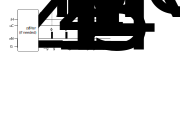
\includegraphics[]{pp/hmbc_15n.png}%
    \caption[NOAH \nitrogen{} HMBC module]{
        NOAH \nitrogen{} HMBC module.
        The $zz$-filter can be implemented as necessary in the same way as for the \carbon{} HMBC module (a final \proton{} \ang{180} pulse may also be required, but is not shown here).
        Delays are set as follows: $\Delta_{\ch{N}} = 1 / (2 \cdot \oneJ{NH})$; $\Delta_{\text{LR},\ch{N}} = 1 / (2 \cdot \nJ{NH})$.
        Phase cycling is performed using $\phi_1 = \phi_\text{rec} = (x, -x)$ and $\phi_2 = (x, x, -x, -x)$.
        Gradient amplitudes are $(g_1, g_2, g_3, g_4) = (5\%, 70\%, 30\%, 50.1\%)$.
    }
    \label{fig:noah_15n_hmbc}
\end{figure}

\subsection{ADEQUATE}
\label{subsec:noah__adequate}

Recent stuff.


\section{Solvent suppression in NOAH}
\label{sec:noah__solvsupp}

GENESIS paper.

\section{Parallel and generalised NOAH supersequences}
\label{sec:noah__parallel}

To conclude this chapter, I discuss how \textit{multiple} NOAH supersequences may be run in parallel in order to obtain yet more data from a single experiment.
As of the time of writing, current software limitations in TopSpin limit the \texttt{NBL} parameter (the number of memory blocks) to 5.
This makes it presently impossible to extend a supersequence linearly beyond five modules.
However, it is possible to \textit{interleave} different supersequences, such that one $t_1$ increment of supersequence A is acquired, followed by one $t_1$ increment of supersequence B, before the value of $t_1$ is increased for both supersequences.
In this text, I refer to this as a `vertical' stacking of modules (as opposed to the traditional NOAH concept, which focuses on `horizontal' concatenation of modules).

\subsection{Parallel NOAH supersequences}
\label{sec:noah__parallel_parallel}

\begin{figure}[!htbp]
    \centering
    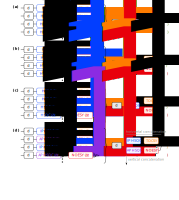
\includegraphics[draft=false]{noah/parallel_noah_overview.png}%
    {\phantomsubcaption\label{fig:parallel_noah_overview_conv}}%
    {\phantomsubcaption\label{fig:parallel_noah_overview_interleaved}}%
    {\phantomsubcaption\label{fig:parallel_noah_overview_kscaled}}%
    {\phantomsubcaption\label{fig:parallel_noah_overview_parallel}}%
    \caption[Overview of parallel NOAH supersequences]{
        An overview of `parallel' NOAH supersequences.
        The left side of each diagram explicitly spells out how $t_1$ is incremented for each module: the value in parentheses indicates the current value of $t_1$, which begins at 0 and is incremented by $\Delta t_1$ each time.
        The right side is a `condensed' depiction of the entire supersequence.
        \textbf{(\subref*{fig:parallel_noah_overview_conv})} A `standard' NOAH supersequence, where $t_1$ for every module is incremented at the same time.
        \textbf{(\subref*{fig:parallel_noah_overview_interleaved})} The first example of a `parallel' supersequence: the HSQC module is acquired as normal, but the TOCSY and NOESY modules are interleaved in the second slot.
        \textbf{(\subref*{fig:parallel_noah_overview_kscaled})} The same as in (\subref*{fig:parallel_noah_overview_interleaved}), but the HSQC module is subjected to $k$-scaling (see also \cref{subsec:noah__hmqc}).
        \textbf{(\subref*{fig:parallel_noah_overview_parallel})} A fully parallel supersequence, where both the first and second module slots are varied systematically.
        This amounts to the interleaved acquisition of two different `standard' supersequences.
    }
    \label{fig:parallel_noah_overview}
\end{figure}

This concept is more clearly illustrated in \cref{fig:parallel_noah_overview}, which contains a more explicit depiction of how $t_1$ is incremented for each module.
In \cref{fig:parallel_noah_overview_conv}, a `traditional' \noah{S,T} supersequence is shown: here, $t_1$ is incremented for both the HSQC and TOCSY module at the same time, and on each $t_1$ increment, the sequence of modules being acquired is always the same.
In \cref{fig:parallel_noah_overview_interleaved}, this is different: the second module is alternated between a TOCSY and a NOESY.
If the total experimental duration (which is largely proportional to the number of recovery delays, $d_1$) is to be kept the same as before, this means that the TOCSY and NOESY modules will be recorded with half the number of $t_1$ increments each.%
\footnote{The data must also be separated prior to Fourier transformation in the indirect dimension. This is `just' an implementation detail, but \textit{did} require the \texttt{splitx\_au} script to be substantially reworked.}
Although this loss of resolution may be considered a drawback, this scheme does allow us greater \textit{flexibility} in the design of NOAH supersequences: it is not ideal to acquire both a TOCSY and a NOESY using a traditional `linear' supersequence, since both of these modules depend on \magnnot{C} magnetisation.

\Cref{fig:parallel_noah_overview_kscaled} shows how the different $F_1$ resolutions can be `fixed' by performing the equivalent of $k$-scaling on the HSQC module (described in \cref{subsec:noah__hmqc}).
This entails reducing the number of $t_1$ increments by a factor of 2 (in this case), and acquiring each increment twice instead, which corresponds to a doubling of the number of scans after the data have been appropriately combined.
This generally has very little impact on the spectra (as was previously shown), but provides a convenient lead into the final example of \cref{fig:parallel_noah_overview_parallel}.
Here, instead of acquiring each increment of the HSQC module twice, the time is used to acquire two different modules, an in-phase (IP) and antiphase (AP) HSQC (both run without \carbon{} decoupling).
Through appropriate linear combination of the data, it is possible to isolate the two peaks of the \proton{}--\carbon{} doublets in these spectra, and from thence measure $\oneJ{CH}$ values: this is known as in-phase/antiphase (IPAP) processing.\autocite{Ottiger1998JMR,Nolis2006JMR,Enthart2008JMR,Gil2010JMR}
Much like the TOCSY and NOESY combination, it is not possible to acquire IP and AP HSQC spectra in a single, linear supersequence, not even with the partial \magn{C} excitation technique described in \cref{subsec:noah__hsqctocsy}.
For the IPAP processing to work, the IP and AP spectra have to be acquired with the same intensity for all peaks: even with a careful choice of $f$ in a linear supersequence, it is not possible to ensure this.

The reader will no doubt notice at this point that \cref{fig:parallel_noah_overview_parallel} corresponds simply to the interleaved acquisition of two different supersequences (one is IP-HSQC + COSY, and the other AP-HSQC + NOESY), which could just as well be acquired separately.
Furthermore, both supersequences are acquired with only half the usual $F_1$ resolution (assuming the same experimental time as \cref{fig:parallel_noah_overview_conv}), meaning that there are \textit{no real time savings}.
This is indeed correct: fundamentally, `vertical' stacking does not increase the number of FIDs recorded per recovery delay, so does not improve the time efficiency (or $\rho_t$).
The main benefits of this process are, in my opinion:
\begin{itemize}
    \item the \textit{flexibility} to construct supersequences that combine previously incompatible modules (such as in the examples above); and
    \item a way of \textit{adjusting for relative sensitivities of different modules}.
        For example, the arrangement in \cref{fig:parallel_noah_overview_kscaled} amounts to the acquisition of the HSQC module for $2n$ scans, and the TOCSY and NOESY modules for $n$ scans each (where $n$ is some positive integer).
        In this way, less intrinsically sensitive modules can be assigned a larger number of scans, such that all modules in the supersequence have (relatively) equalised intensities.
\end{itemize}

In principle, all of the above may still be accomplished in a roundabout manner by acquiring multiple separate supersequences and then combining the results.
This is most obvious in \cref{fig:parallel_noah_overview_parallel}.
However, the current implementation of parallel supersequences provides \textit{convenience} for the user, as all experiments may be simultaneously acquired and processed.
This factor should not be overlooked, especially considering that all the different constructions (\cref{fig:parallel_noah_overview_interleaved,fig:parallel_noah_overview_kscaled,fig:parallel_noah_overview_parallel}) must be processed in a slightly different manner: it is easier to do this from within a single experiment, rather than attempting to combine FIDs from separate datasets after the fact.
There is also another argument for acquiring increments in an interleaved manner: this helps to minimise drifts in the spectra which arise from temporal instabilities in (for example) temperature.

\begin{figure}[!ht]
    \centering
    \includegraphics[draft=false]{noah/tsnoah_example.png}%
    {\phantomsubcaption\label{fig:tsnoah_example_overall}}%
    {\phantomsubcaption\label{fig:tsnoah_example_b1}}%
    {\phantomsubcaption\label{fig:tsnoah_example_b2}}%
    {\phantomsubcaption\label{fig:tsnoah_example_sc1}}%
    {\phantomsubcaption\label{fig:tsnoah_example_sc2}}%
    {\phantomsubcaption\label{fig:tsnoah_example_s1}}%
    {\phantomsubcaption\label{fig:tsnoah_example_s2}}%
    {\phantomsubcaption\label{fig:tsnoah_example_cc}}%
    {\phantomsubcaption\label{fig:tsnoah_example_t}}%
    \caption[Spectra from a NOAH-8 `parallel' supersequence]{
        \textbf{(\subref*{fig:tsnoah_example_overall})} Condensed representation of the supersequence, which may be interpreted in the same way as \cref{fig:parallel_noah_overview_parallel}.
        \textbf{(\subref*{fig:tsnoah_example_b1})} HMBC, optimised for $\nJ{CH} = \qty{5}{\Hz}$.
        \textbf{(\subref*{fig:tsnoah_example_b2})} HMBC, optimised for $\nJ{CH} = \qty{10}{\Hz}$.
        \textbf{(\subref*{fig:tsnoah_example_sc1})} IP HSQC-CLIP-COSY.
        \textbf{(\subref*{fig:tsnoah_example_sc2})} AP HSQC-CLIP-COSY.
        \textbf{(\subref*{fig:tsnoah_example_s2})} IP multiplicity-edited seHSQC.
        \textbf{(\subref*{fig:tsnoah_example_s2})} AP multiplicity-edited seHSQC.
        \textbf{(\subref*{fig:tsnoah_example_cc})} CLIP-COSY.
        \textbf{(\subref*{fig:tsnoah_example_t})} TOCSY (\qty{60}{\ms} mixing time).
    }
    \label{fig:tsnoah_example}
\end{figure}

\Cref{fig:tsnoah_example_overall} shows one example of a more complex parallel supersequence containing 8 modules.
In this supersequence, the HMBC module is recorded twice with the delay $\Delta_\text{LR}$ optimised for two different values of $\nJ{CH}$ (\cref{fig:tsnoah_example_b1,fig:tsnoah_example_b2}): these spectra furnish a (slightly) different set of correlations, which allow for more complete structure determination.
The HSQC-CLIP-COSY is acquired in an IPAP fashion, where direct/indirect editing is used in one experiment (\cref{fig:tsnoah_example_sc2}) and not in the other (\cref{fig:tsnoah_example_sc1}).
Likewise, the $F2$-coupled seHSQC experiment is also performed in an IPAP manner, where this time the `IPAP' components are the two peaks in each doublet.
Multiplicity editing is additionally used here in both IP and AP seHSQC spectra.
Finally, we have two interleaved homonuclear modules, the CLIP-COSY and TOCSY (\cref{fig:tsnoah_example_cc,fig:tsnoah_example_t}), which provide complementary information about spin networks.
The four IPAP-processed spectra from this supersequence are shown in \cref{fig:tsnoah_ipap_spec}.

\begin{figure}[!ht]
    \centering
    \includegraphics[draft=false]{noah/tsnoah_ipap_spec.png}%
    {\phantomsubcaption\label{fig:tsnoah_ipap_spec_sc_direct}}%
    {\phantomsubcaption\label{fig:tsnoah_ipap_spec_sc_indirect}}%
    {\phantomsubcaption\label{fig:tsnoah_ipap_spec_s_alpha}}%
    {\phantomsubcaption\label{fig:tsnoah_ipap_spec_s_beta}}%
    \caption[IPAP processed spectra from NOAH-8 supersequence]{
        \textbf{(\subref*{fig:tsnoah_ipap_spec_sc_direct})--(\subref*{fig:tsnoah_ipap_spec_sc_indirect})} IPAP-processed HSQC-COSY spectra (from \cref{fig:tsnoah_example_sc1,fig:tsnoah_example_sc2}), which separate the `direct' and `indirect' HSQC-COSY responses described in \cref{subsec:noah__hsqccosy}.
        \textbf{(\subref*{fig:tsnoah_ipap_spec_s_alpha})--(\subref*{fig:tsnoah_ipap_spec_s_beta})} IPAP-processed seHSQC spectra (from \cref{fig:tsnoah_example_s1,fig:tsnoah_example_s2}), each of which contain one peak of each \proton{}--\carbon{} doublet.
    }
    \label{fig:tsnoah_ipap_spec}
\end{figure}

\subsubsection{Time-shared NMR}

In my published work\autocite{Kupce2021JACSA}, what I refer to as IPAP here is frequently labelled as a TS, or \textit{time-shared} experiment.
In TS NMR, pulse sequences are specially designed in order to record two (or more) different signals at once, such as a \carbon{} HSQC and a \nitrogen{} HSQC: this has found use in both biomolecular\autocite{Farmer1991JMR,Boelens1994JBNMR,Pascal1994JMRSB,Sattler1995JBNMR,Frueh2009JBNMR,Lohr2014JMR} and small-molecule NMR\autocite{Nolis2006MRC,PerezTrujillo2007OL,Nolis2007ACIE,Parella2010CMR}.
Often, the design of TS experiments involves the joint evolution of both heteronuclear chemical shifts in a shared $t_1$ period: hence the term `time-shared'.

It should be noted that TS experiments use \textit{simultaneous} acquisition, as opposed to the \textit{sequential} acquisition of NOAH experiments.
In other words, the two or more signals recorded in a TS experiment are part of the same FID, meaning that the resulting spectra will contain peaks from both signals.
If these can be easily disambiguated (e.g.\ by the differing chemical shifts of \carbon{}- or \nitrogen{}-bonded protons), then the TS experiment allows more data to be collected in the same amount of time as a non-TS experiment.
However, if these signals must be separated, then the TS experiment must be repeated: once where the two signals have the same phase, and once where they have opposite phases.
The underlying signals can then be disentangled through linear combination.\autocite{Sorensen1990JMR,Farmer1991JMR}

Mathematically, this is exactly the same process as IPAP processing.
In my view, what separates the two is the fact that the IPAP technique seeks to disentangle components which are \textit{innate} to the pulse sequence under consideration and cannot usually be isolated---such as doublets in a $F_2$-coupled HSQC---whereas TS experiments must be \textit{specially crafted} to record these multiple components.
Equivalently, the time savings (or sensitivity improvement) from a TS experiment stem from the fact that it is being compared against a pair of experiments which each yield only one of the two signals detected in the TS sequence.

In this case, the IPAP label clearly applies to the pair of $F_2$-coupled seHSQC modules in \cref{fig:tsnoah_example_s1,fig:tsnoah_example_s2}.
However, for the HSQC-COSY modules in \cref{fig:tsnoah_example_sc1,fig:tsnoah_example_sc2}, the situation is less clear.
The two `signals' which we should consider are the `direct' and `indirect' peaks; however, it is not entirely obvious which experiments can be used for these.
The `direct' peaks correspond to a (\carbon{}-decoupled) HSQC experiment.%
\footnote{It should be noted that the intensities of the direct peaks in an HSQC-COSY spectrum are lower than in the corresponding HSQC spectrum, because the direct peaks in an HSQC-COSY stem only from magnetisation which does \textit{not} evolve under $\nJ{HH}$ during the mixing period. However, TS experiments do generally have lower sensitivity than the non-TS counterparts, so this is not really an issue.}
However, for the `indirect' peaks, there is no real equivalent spectrum to be compared against: the H2BC experiment\autocite{Nyberg2005JACS,Nyberg2005MRC} yields a similar set of peaks, but in this experiment, the `direct' peaks have in fact been intentionally suppressed through the application of a LPJF.
When the LPJF is removed (as in the 2BOB/H2OBC experiments\autocite{Kupce2017MRC}), a similar information content to the HSQC-COSY is obtained.
So, it is not entirely accurate to write that the HSQC-COSY combines a HSQC plus H2BC spectrum.
Consequently, I personally prefer to view it as an IPAP experiment.

Of course, the analysis above is only applicable to the modules shown in \cref{fig:tsnoah_example}.
None of this precludes the application of \textit{true} time-shared experiments to NOAH supersequences: it is completely possible to implement, for example, a \carbon{}/\nitrogen{} TS experiment within the context of a parallel supersequence.
However, many TS experiments are already designed to detect signals arising from different magnetisation pools (e.g.\ \magn{C} and \magn{N}).
This is already something which can be accomplished in a cleaner manner using (linear) NOAH supersequences.



\subsection{Generalised supersequences}
\label{sec:noah__parallel_generalised}

From the discussion above, it is evident that there is no need to stop at \textit{two} interleaved modules: it is possible to endlessly stack modules in a vertical manner.
Furthermore, different modules may be acquired a different number of times.
Thus, in \cref{fig:parallel_noah_overview_interleaved}, two supersequences were interleaved, and the TOCSY and NOESY modules were acquired once each in each $t_1$ increment.
However, if $M$ different supersequences are being interleaved, then a set of two different modules may be acquired $m_1$ and $m_2$ times, as long as $m_1 + m_2 = M$.
For example, a supersequence with $m_1 = 1$ and $m_2 = 3$ is shown in \cref{fig:generalised_example}.
Generally, it is desirable to assign larger $m_i$ values to less sensitive modules, as the results can be summed up to yield improved signal-to-noise.

\begin{figure}[!ht]
    \centering
    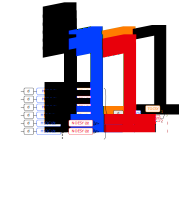
\includegraphics[draft=false]{noah/generalised_example.png}%
    \caption[A basic example of a generalised supersequence]{
        A basic example of a `generalised' NOAH supersequence, where an arbitrary number of supersequences (here three) can be vertically `stacked'.
        For each value of $t_1$, the TOCSY is acquired once, the NOESY twice, and the HSQC three times, as indicated by the subscripts in the condensed representation on the right.
    }
    \label{fig:generalised_example}
\end{figure}

\subsubsection{Pulse sequence implementation}

Unfortunately, GENESIS is not (at present) advanced enough to create pulse programmes generalised supersequences.
Thus, the pulse programmes for this section have been written by hand.
The overall structure of such a pulse programme is shown in \cref{lst:generalised_pp}.
The parameter \texttt{CNST51} corresponds to the number of supersequences being interleaved, i.e., $M$ in the discussion above.
The values of $m_1$ and $m_2$ are encoded as \texttt{CNST52} and \texttt{CNST53}; the latter of these can be automatically calculated.

\begin{mylisting}[!htbp] % lst:generalised_pp {{{1
\begin{tcbminted}{bruker}
"l0     = td1/2"             ; TD1/NBL
"cnst53 = cnst51 - cnst52"   ; automatically calculate m_2 = M - m_1
; ...

1 ze
2 30m
4 50u UNBLKGRAD
  d1 st0

  ; HSQC goes here
  ; ...
  goscnp ph30 cpd2:f2
  50u do:f2

  ; check which module to run
  if "l3 % cnst51 < cnst52"
{
  ; TOCSY goes here
  ; ...
  go=2 ph31
}
  else
{
  ; NOESY goes here
  ; ...
  go=2 ph31
}

  ; move to next 'row' in diagram
  1m iu3
  30m wr #0 if #0 zd

  ; check if M 'rows' have passed
  if "l3 % cnst51 == 0"
{
  1m iu1
  1m igrad EA   ; HSQC echo-antiecho gradients
  ; ...
}

  lo to 4 times l0
end
\end{tcbminted}
    \caption[Structure of pulse programme for generalised supersequences]{
        The overall structure of the pulse programme for the generalised supersequence in \cref{fig:generalised_example}.
    }
    \label{lst:generalised_pp}
\end{mylisting} % }}}1

This structure provides a clear blueprint for how GENESIS can be adapted to produce generalised supersequences.
The only thing which GENESIS needs to detect is how many modules are being interleaved, which determines the number of $m_i$'s.
It should be noted that the `parallel' supersequence of \cref{fig:parallel_noah_overview_kscaled} can be obtained by setting $M = 2$ and $m_1 = m_2 = 1$, and standard linear supersequences simply have $M = m_1 = 1$.
Thus, if generalised supersequences were to be implemented in GENESIS, all other types of supersequences can be obtained `for free'.

A small technical detail in \cref{lst:generalised_pp} is that each \texttt{go=2} statement loops back to the label \texttt{2}, such that the experiment is repeated \texttt{NS} times.
This means that in the left side of \cref{fig:generalised_example}, each row is already acquired a total of \texttt{NS} times, in addition to any repetition which is explicitly shown.
Thus, after summation of the explicitly repeated increments, the HSQC will in fact end up with a total of \texttt{3*NS} scans.
However, the \textit{phase cycle} is only moved forward within the \texttt{NS} loop; each time \texttt{NS} repetitions are completed, the phase cycle is reset to the beginning.
This means that even though each FID in the HSQC is acquired \texttt{3*NS} times, only an \texttt{NS}-step phase cycle is used.
Thus, in order to obtain spectra of the highest possible quality, any common divisors of $M$ and the $m_i$'s should be factorised out and placed into \texttt{NS} instead.


\subsubsection{Examples}

\begin{figure}[!ht]
    \centering
    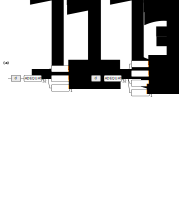
\includegraphics[draft=false]{noah/abbs_pp.png}%
    {\phantomsubcaption\label{fig:abbs_pp_abbs}}%
    {\phantomsubcaption\label{fig:abbs_pp_abbss}}%
    \caption[Examples of generalised supersequences]{
        Two examples of generalised NOAH supersequences.
        \textbf{(\subref*{fig:abbs_pp_abbs})} A \noah{A,Bn,B,S} supersequence.
        \textbf{(\subref*{fig:abbs_pp_abbss})} A \noah{A,Bn,B,S,Spn} supersequence.
    }
    \label{fig:abbs_pp}
\end{figure}

Since generalised supersequences allow the effective number of scans to be individually customised for each module, they offer an avenue for modules with (very) different intrinsic sensitivities to be combined.
On the very-low-sensitivity end are spectra such as ADEQUATE and \nitrogen{} HMBC; compared to these, the HSQC experiments may be considered high-sensitivity.
It should be reiterated that the time savings to be obtained through this combination ($\rho_t$) are still on the order of 2, because only two modules are being horizontally concatenated at a time.


\begin{figure}[!htb]
    \centering
    \includegraphics[draft=false]{noah/abbs_spec.png}%
    {\phantomsubcaption\label{fig:abbs_spec_a}}%
    {\phantomsubcaption\label{fig:abbs_spec_bn}}%
    {\phantomsubcaption\label{fig:abbs_spec_b}}%
    {\phantomsubcaption\label{fig:abbs_spec_s}}%
    \caption[Spectra from \noah{A,Bn,B,S} generalised supersequence]{
        Spectra from the \noah{A,Bn,B,S} generalised supersequence (\cref{fig:abbs_pp_abbs}).
        \textbf{(\subref*{fig:abbs_spec_a})} ADEQUATE.
        \textbf{(\subref*{fig:abbs_spec_bn})} \nitrogen{} HMBC, optimised for an $\nJ{NH}$ value of \qty{8}{\Hz}.
        \textbf{(\subref*{fig:abbs_spec_b})} \carbon{} HMBC, optimised for an $\nJ{CH}$ value of \qty{8}{\Hz}.
        \textbf{(\subref*{fig:abbs_spec_s})} \carbon{} HSQC.
        \datacode{7X-220604}
    }
    \label{fig:abbs_spec}
\end{figure}

\begin{figure}[!ht]
    \centering
    \includegraphics[draft=false]{noah/abbss_spec.png}%
    {\phantomsubcaption\label{fig:abbss_spec_a}}%
    {\phantomsubcaption\label{fig:abbss_spec_bn}}%
    {\phantomsubcaption\label{fig:abbss_spec_b}}%
    {\phantomsubcaption\label{fig:abbss_spec_s}}%
    {\phantomsubcaption\label{fig:abbss_spec_sn}}%
    \caption[Spectra from \noah{A,Bn,B,S,Spn} generalised supersequence]{
        Spectra from the \noah{A,Bn,B,S,Spn} generalised supersequence (\cref{fig:abbs_pp_abbss}).
        \textbf{(\subref*{fig:abbss_spec_a})} ADEQUATE.
        \textbf{(\subref*{fig:abbss_spec_bn})} \nitrogen{} HMBC, optimised for an $\nJ{NH}$ value of \qty{4}{\Hz}.
        \textbf{(\subref*{fig:abbss_spec_b})} \carbon{} HMBC, optimised for an $\nJ{CH}$ value of \qty{8}{\Hz}.
        \textbf{(\subref*{fig:abbss_spec_sn})} \nitrogen{} seHSQC.
        \textbf{(\subref*{fig:abbss_spec_s})} \carbon{} HSQC.
        \datacode{7C-220722}
    }
    \label{fig:abbss_spec}
\end{figure}

\Cref{fig:abbs_pp} shows some examples of such experiments, where the relative numbers of scans are chosen with the aim of balancing the sensitivities of each module.
The ADEQUATE module used here is the ZIP-ADEQUATE experiment shown in \cref{fig:adequate_noah}; this consumes \magn{C} magnetisation and preserves the \magnnot{C} magnetisation required by the \nitrogen{} HMBC, \carbon{} HMBC, and \nitrogen{} seHSQC.
However, the \carbon{} HSQC module draws on the same magnetisation pool; therefore, in order to maximise the intensities in this experiment, a period of isotropic mixing is applied only before the HSQC module in order to effect polarisation transfer from \magnnot{C} spins.
The spectra thus obtained are shown in \cref{fig:abbs_spec,fig:abbss_spec}.

Another additional implementation detail, related to the earlier point about phase cycling, is that on each repetition of the ADEQUATE/\nitrogen{} HMBC increments, the \nitrogen{} HMBC signal (specifically, the first \nitrogen{} \ang{90} pulse) and receiver phases are additionally inverted.
This can be accomplished by adding the corresponding extra phase incrementation instructions just underneath the \texttt{1m iu3} line in \cref{lst:generalised_pp}, and can be thought of as a form of `manual' phase cycling, which is independent of (and complementary to) the usual phase cycle specified in the pulse programme.
The reason for doing this is to suppress artefacts which appear at $F_1 \approx 0$ in the \nitrogen{} HMBC, which stem from the ADEQUATE module (when the \nitrogen{} HMBC is run on its own, these artefacts do not appear).
The exact origin of these artefacts is still unclear,%
\footnote{Their frequencies in $F_1$ are not exactly zero, so there is \textit{some} kind of modulation in the $t_1$ period of the ADEQUATE module, but it is not entirely clear where this is happening. My current best guess is that the offending magnetisation evolves during the constant-time period of the ADEQUATE, where the double-quantum frequencies are reconverted into single-quantum frequencies.}
but their phase is constant; thus, inverting the \nitrogen{} HMBC receiver phase leads to their cancellation.
It should be noted that the issue of phase cycling is not unique to generalised supersequences: indeed, such phase cycling would also be necessary in a standard linear \noah{A,Bn} supersequence.
However, because the degree of built-in phase cycling in a generalised supersequence is lower than the actual number of transients recorded for each module, some of it must be explicitly specified in this way.


\subsubsection{Covariance analysis}

The generalised supersequences shown in \cref{fig:abbs_pp,fig:abbs_spec,fig:abbss_spec} yield very thorough information about heteronuclear connectivity, including one-bond and long-range \proton{}--\carbon{} and \proton{}--\nitrogen{} couplings.
These spectra can be used as inputs for indirect covariance processing\autocite{Zhang2004JACS,Snyder2009JPCA,Jaeger2014ARNMRS} in order to yield `unnatural' (but very informative) double heteronuclear correlation spectra, in which each peak represents a correlation between two dilute heteronuclei (\carbon{} or \nitrogen{}).
Directly recording such spectra through an NMR experiment would require substantially more time, because of the extremely low probability of finding two heteronuclei in the same isotopologue.

Some possible covariance spectra obtained from the data in \cref{fig:abbs_spec,fig:abbss_spec} are shown in \cref{fig:covariance_spec}.
All covariance calculations were performed in Python, according to the formulae:
\begin{equation}
    \label{eq:covariance_unsymmetrical}
    \symbf{C} = \symbf{S}_1\symbf{S}_2^T
\end{equation}
for unsymmetrical indirect covariance (where $\symbf{S}_1$ and $\symbf{S}_2$ are the input spectra and $\symbf{C}$ the covariance spectrum), or
\begin{equation}
    \label{eq:covariance_generalised}
    \symbf{M} = \left[\begin{pmatrix}\symbf{S}_1 \\ \symbf{S}_2\end{pmatrix}
    \begin{pmatrix}\symbf{S}_1 & \symbf{S}_2 \end{pmatrix}\right]^\lambda
\end{equation}
for generalised indirect covariance; the covariance spectrum $\symbf{C}$ can then be obtained as an off-diagonal block of the matrix $\symbf{M}$.
$\lambda$ is a parameter which is chosen in order to balance peak intensity and artefact intensity\autocite{Snyder2009JPCA}.

In \cref{fig:covariance_spec_bruc_cn}, the brucine \nitrogen{} HMBC and \carbon{} HSQC spectra  (\cref{fig:abbs_spec_bn,fig:abbs_spec_s}) are processed using unsymmetrical indirect covariance to yield a \carbon{}--\nitrogen{} correlation spectrum which contains both one- and long-range correlations.\autocite{Martin2007JHC,Martin2007MRC}
The sign of the peaks indicates the multiplicity of the \carbon{} involved, and stems from the use of multiplicity editing in the \carbon{} HSQC spectrum.
Unfortunately, one of the weaknesses of covariance spectra is on show here: there are several artefacts in this spectrum (marked by asterisks), caused by overlap in the \proton{} dimension of both input spectra.

The other three spectra (\cref{fig:covariance_spec_cyclo_caco,fig:covariance_spec_cyclo_cacb_nosymm,fig:covariance_spec_cyclo_cacb_symm}) combine the cyclosporin \carbon{} HSQC and ADEQUATE modules (\cref{fig:abbss_spec_a,fig:abbss_spec_s}) to generate a \carbon{}--\carbon{} one-bond correlation spectrum: essentially, an INADEQUATE spectrum (but with single-quantum frequencies in both dimensions)\autocite{Martin2011MRC,Martin2011MRC2}.
This should in principle be symmetric about the main diagonal.
However, since the HSQC only detects protonated carbons, and the ADEQUATE input spectrum only detects correlations involving at least one protonated carbon.
Thus, correlations between two quaternary carbons do not appear, and correlations between protonated and quaternary carbons only appear once in the spectrum (instead of twice).
This does not a problem in the case of cyclosporin, though, as the only quaternary carbons are those of the carbonyl (\ch{CO}) group, which will still display correlations to the adjacent \ch{C}$\alpha$ carbons.

These \ch{C}$\alpha$--\ch{CO} correlations are shown in \cref{fig:covariance_spec_cyclo_caco}.
There are 11 peaks here, one for each amino acid residue in cyclosporin: again, the sign indicates the \ch{C}$\alpha$ multiplicity (all are \ch{CH} except for the \textit{N}-methylglycine \ch{CH2}).
In \cref{fig:covariance_spec_cyclo_cacb_nosymm,fig:covariance_spec_cyclo_cacb_symm}, the \ch{C}$\alpha$--\ch{C}$\beta$ correlations are shown.
This part of the spectrum has been further subjected to a sign-preserving symmetrisation procedure, where the intensity at each point $p(\Omega_1, \Omega_2)$ is replaced by
\begin{equation}
    \label{eq:covariance_symmetrisation}
    p(\Omega_1, \Omega_2) = \sgn[p(\Omega_1, \Omega_2)] \cdot \min\left\{|p(\Omega_1, \Omega_2)|, |p(\Omega_2, \Omega_1)|\right\}.
\end{equation}
Here, $\sgn{x}$ refers to the sign of $x$, or equivalently $x / |x|$ (for $x \neq 0$).
Since all \ch{C}$\alpha$ and \ch{C}$\beta$ carbons in cyclosporin are protonated, the spectrum is expected to be symmetric; this symmetrisation process therefore helps to remove some of the artefacts which tend to plague the interpretation of covariance spectra.

\begin{figure}[!ht]
    \centering
    \includegraphics[draft=false]{noah/covariance.png}%
    {\phantomsubcaption\label{fig:covariance_spec_bruc_cn}}%
    {\phantomsubcaption\label{fig:covariance_spec_cyclo_caco}}%
    {\phantomsubcaption\label{fig:covariance_spec_cyclo_cacb_nosymm}}%
    {\phantomsubcaption\label{fig:covariance_spec_cyclo_cacb_symm}}%
    \caption[Examples of covariance spectra obtained from generalised NOAH supersequences]{
        Examples of covariance spectra obtained from generalised NOAH supersequences.
        \textbf{(\subref*{fig:covariance_spec_bruc_cn})} \carbon{}--\nitrogen{} correlation spectrum for brucine.
        Asterisks indicate artefacts arising from peak overlap.
        \textbf{(\subref*{fig:covariance_spec_cyclo_caco})} Inset of the \carbon{}--\carbon{} one-bond correlation spectrum for cyclosporin, obtained by processing the ADEQUATE and \carbon{} HSQC spectra in \cref{fig:abbss_spec_a,fig:abbss_spec_s} using generalised indirect covariance ($\lambda = 0.5$).
        The region shown here contains correlations between \ch{CO} and \ch{C}$\alpha$ carbons.
        \textbf{(\subref*{fig:covariance_spec_cyclo_cacb_nosymm})--(\subref*{fig:covariance_spec_cyclo_cacb_symm})} A different inset from the same \carbon{}--\carbon{} correlation spectrum as in (\subref*{fig:covariance_spec_cyclo_caco}), but this time showing correlations in the alkyl region.
        The spectrum in (\subref*{fig:covariance_spec_cyclo_cacb_symm}) has been further subject to a sign-preserving symmetrisation process.
        The \ch{CO}--\ch{C}$\alpha$ and \ch{C}$\alpha$--\ch{C}$\beta$ correlations for all residues are labelled in (\subref*{fig:covariance_spec_cyclo_caco}) and (\subref*{fig:covariance_spec_cyclo_cacb_symm}) (following the numbering in \todo{REF}).
    }
    \label{fig:covariance_spec}
\end{figure}

\section{Conclusion}
\label{sec:noah__conclusion}

In this chapter, I covered a variety of improvements to NOAH supersequences, including the development of new or improved modules (\cref{sec:noah__modules}), the implementation of basic solvent suppression (\cref{sec:noah__solvsupp}), and the generalised NOAH sequences obtained through `vertical stacking' of different supersequences (\cref{sec:noah__parallel}).

As a technique in fast 2D NMR, NOAH is in my view fairly mature despite its relative recency (the first paper was published in 2017\autocite{Kupce2017ACIE}).
The underlying idea of separating magnetisation pools, and the tools used to do so, have been around for quite a while---most recently, and notably, in the form of ASAP 2D NMR.
Thus, rather than making fundamental conceptual breakthroughs, I would characterise my work here as `polishing the remaining rough edges', whether by removing artefacts or by incorporating slightly more specialised modules.

Naturally, the possibility of using the same concept to accelerate 3D (or higher) experiments is extremely attractive.
Some of the ground work for this has already been laid, in the form of ASAP-type 3D experiments.\autocite{Schanda2009PNMRS}
However, my opinion is that this research topic would extend far beyond NOAH itself: in particular, 3D experiments are often applied to isotopically labelled substances, which lead to a different set of magnetisation pools which are not so easily separable.

At this point, assuming that there are few fundamental breakthroughs to be made in NOAH itself, we must turn to the question of how to increase its uptake.
The accessibility of new techniques is \textit{always} a significant factor, regardless of the merit of the underlying technique.
For this reason, I am particularly proud of the GENESIS website (\cref{sec:noah__genesis}) and the associated improvements in the processing pipeline; the feedback from the NMR community has also been greatly encouraging.
At the same time, there is still some way to go: although one may consider a `standard' NOAH experiment easy enough to set up, after taking into account other desirable features such as automation and NUS, the entire process can become rather non-trivial.

Another important, but under-explored, area is the use of NOAH in the sensitivity-limited regime.
The results in this chapter are derived from samples which are not particularly dilute, and hence belong in the resolution-limited regime.
While this may lead to a maximisation of the \textit{relative} (in that $\rho_t > \rhoteff$), the \textit{absolute} time savings are small because the standalone 2D experiments would be completed fairly quickly anyway.
This is particularly relevant for (e.g.) unstable samples, for which 2D data need to be acquired in as short a time as possible.
Conclusively demonstrating the benefits of NOAH experiments on such samples would go a long way towards convincing more synthetic chemists to adopt the NOAH technique.



\printbibliography[heading=subbibnumbered]{}
